\documentclass[10pt,a4paper]{article}
\usepackage[margin=0.75in]{geometry}
\usepackage[T1]{fontenc}
\usepackage[utf8]{inputenc}
\usepackage{lmodern,amsmath,amssymb,booktabs,array,enumitem}
\usepackage[expansion=false]{microtype}
\usepackage{csquotes}
\usepackage{xurl,hyperref,pdflscape,tabularx,algorithm,algpseudocode,graphicx,tikz,xcolor}
\usepackage[section]{placeins}
\usepackage{caption}
\captionsetup{font=small,labelfont=bf}
\setlength{\emergencystretch}{1.5em}
\raggedbottom
\hypersetup{hidelinks,pdftitle={Phase 2: Poisoning, Retention and Legitimate Adaptation},pdfauthor={Saneedullah; Ahmed Bilal}}
\newcolumntype{Y}{>{\raggedright\arraybackslash}X}
\newcolumntype{L}[1]{>{\raggedright\arraybackslash}p{#1}}
\newcommand{\NA}{\mathrm{N/A}}
\newcommand{\CE}{\operatorname{CE}}
\newcommand{\sumitem}[2]{\noindent\textbf{#1:} #2\par}
\newcommand{\why}[1]{\par\nopagebreak[4]\noindent\colorbox{black!5}{\parbox{\dimexpr\linewidth-2\fboxsep}{\small\textbf{Why (literature basis):} #1}}\par}
\setlength{\parindent}{0pt}
\setlength{\parskip}{4pt}
\setlength{\tabcolsep}{3pt}
\setlength{\intextsep}{8pt}
\renewcommand{\arraystretch}{1.12}
\setlist{nosep,leftmargin=*}

\title{\textbf{Computer Networks --- Research Project}\\[4pt]
\large Phase 2: Extended Literature Review and Research Methodology\\[8pt]
\Large Poisoning, Retention and Legitimate Adaptation\\in Federated Continual Intrusion Detection}
\author{Saneedullah (23I-2568) \qquad Ahmed Bilal (23I-2581)}
\date{October 2026}

\begin{document}
\maketitle

\begin{abstract}
Intrusion detection systems must learn new attack families while retaining earlier knowledge. Federated learning combines updates from multiple sites, creating an opportunity for a corrupted labelling feed to affect the shared model. We extend our Phase 1 review with ten additional 2025--2026 studies. In this selected corpus, continual IDS studies generally evaluate trusted training data, whereas federated poisoning defences use fixed class sets. The joint effect of poisoning during class acquisition, subsequent attacker withdrawal and legitimate adaptation remains insufficiently evaluated. We propose a five-client simulation on CICIDS2017 with four successive attack-family stages, comparing fine-tuning, an EWC-style regulariser and DER++ replay. One client's DoS-Hulk training labels are partly changed to benign during the second stage only. We measure immediate source-family damage and later persistence, and compare class-aware admission with a global filter that admits the same number of records. Acquisition on untargeted new families is evaluated separately from source-family damage. Twelve paired seeds, development-only tuning and a pre-specified analysis support this controlled comparison. This is a research proposal; quoted performance results belong to the cited studies, and null or adverse outcomes remain valid findings.
\end{abstract}

\noindent\textbf{Keywords:} continual learning; federated learning; intrusion detection; label poisoning; replay memory; legitimate adaptation.

%=====================================================================
\section{Introduction and Scope}
Network attacks change continuously. An IDS that is retrained on each new attack family tends to forget earlier families (\emph{catastrophic forgetting}); continual-learning (CL) methods such as regularisation and replay reduce this problem. At the same time, data-governance constraints can motivate organizations to use \emph{federated learning} (FL), where each site trains locally and only model updates are combined. Combining the two creates a security question that neither field answers on its own: what happens when one participant's labels are wrong \emph{while} the shared model is learning a new attack family, and does a defence that filters suspicious data also block the legitimate new family it should learn?

Our Phase 1 report \cite{phase1} studied three 2026 papers on CL for network security \cite{ge,wu,luo} and identified three gaps: old or synthetic evaluation data, no testing against attackers who target the adaptation mechanism, and no measured deployment cost. Phase 2 keeps Phase 1 unchanged and builds on it. Table~\ref{tab:phase1link} shows how each Phase 1 gap is carried forward.

\begin{table}[H]
\centering\footnotesize
\caption{How the Phase 1 gaps carry into Phase 2.}
\label{tab:phase1link}
\begin{tabularx}{\linewidth}{L{4.6cm}L{3.3cm}Y}
\toprule
Phase 1 gap & Phase 2 status & Reason\\
\midrule
Gap 1: old, narrow or synthetic evaluation data & Partly addressed & Historical CICIDS2017 supports controlled tests; CICIoT2023 is a planned extension. Modern multi-site generalisation remains open.\\
Gap 2: no attacker targeting the continual-learning mechanism & \textbf{Retained as the core} & Becomes Gaps G1 and G2 below: poisoning during class acquisition and defence side-effects.\\
Gap 3: no measured runtime or deployment cost & Partly retained & We measure CPU time, memory and update bytes; physical edge-device energy is deferred (no hardware available).\\
\bottomrule
\end{tabularx}
\end{table}

\begin{samepage}
We ask three research questions:
\begin{itemize}
\item \textbf{RQ1:} How do fine-tuning, an EWC-style regulariser and DER++ replay differ in the damage a poisoned stage causes to the targeted attack family, both immediately and after the attacker withdraws?
\item \textbf{RQ2:} Compared with a global filter that admits the same number of samples, how does a class-aware admission rule change the trade-off between poisoning damage and the learning of new attack families?
\item \textbf{RQ3:} Which memory and selection mechanisms explain the differences, and what computation and communication do they cost?
\end{itemize}
\end{samepage}
Throughout this document, page numbers cited for the reviewed articles refer to the PDF pages of each article.

%=====================================================================
\section{Deliverable 1: Extended Literature Review}

\subsection{Search Strategy and Selection Criteria}
We searched for studies that combine at least two of: intrusion detection, continual or incremental learning, federated learning, and poisoning. The corpus was closed on 20 October 2026. Sources were the Crossref publication index (articles published from 1 January 2025 through that cutoff; queries such as \emph{federated continual learning intrusion detection}, \emph{poisoning attack federated intrusion detection defense} and \emph{class incremental intrusion detection replay}), author and publisher pages, and the references of our Phase 1 papers. Each candidate had to satisfy the course criteria: published in 2025--2026; an original research article; a Q1--Q2 journal or a peer-reviewed conference; directly relevant; with an identifiable method, dataset and evaluation. We kept only papers whose \emph{complete} text we could read, because a critical analysis needs the full experimental details. One formally eligible candidate was rejected after full reading because its dataset was synthetic and unpublished and its results came from a single run. Table~\ref{tab:corpus} lists the ten selected papers. Journal quartiles use the \emph{2025 JCR release, based on 2024 JIF data}, consistently across this table \cite{clarivate,jcrtable}. Categories are named because a journal can have different quartiles in different categories. This is a focused, full-text-accessible review, not a systematic review or proof that no other relevant work exists; access and database coverage can bias selection.

\begin{table}[H]
\centering\footnotesize
\caption{The ten additional papers reviewed in Phase 2. CS-IS: Computer Science, Information Systems; EE: Engineering, Electrical and Electronic; II: Instruments and Instrumentation; MS: Multidisciplinary Sciences.}
\label{tab:corpus}
\begin{tabularx}{\linewidth}{L{0.55cm}L{3.3cm}Y L{0.8cm}L{2.9cm}L{2.6cm}}
\toprule
ID & Study & Venue (publisher) & Year & Ranking & Main topic\\
\midrule
P4 & Carillo et al. \cite{carillo} & IEEE Trans. Network and Service Management (IEEE) & 2026 & Q1, CS-IS & Federated class-incremental IDS\\
P5 & Lavaur et al. \cite{lavaur} & Computers \& Security (Elsevier) & 2025 & Q1, CS-IS & Label flipping in federated IDS\\
P6 & Fuhrman et al. \cite{cnd} & ACM/IEEE Design Automation Conf. (DAC) & 2025 & Peer-reviewed conference & Continual novelty detection\\
P7 & Sameera et al. \cite{wei} & J. Information Security and Applications (Elsevier) & 2025 & Q2, CS-IS & Poisoning defence for federated IDS\\
P8 & Cerasuolo et al. \cite{cerasuolo} & Computer Networks (Elsevier) & 2025 & Q1, CS-IS & Class-incremental IDS benchmark\\
P9 & Guo et al. \cite{guo} & Future Internet (MDPI) & 2025 & Q2, CS-IS & Continual IDS, memory selection\\
P10 & Latif and Djenouri \cite{amm} & Sensors (MDPI) & 2026 & Q2, II & Robust hierarchical federated IDS\\
P11 & Banbhrani et al. \cite{flzt} & Electronics (MDPI) & 2026 & Q2, EE & Trust-aware federated IDS\\
P12 & Abhijit et al. \cite{rare} & Scientific Reports (Nature Portfolio) & 2025 & Q1, MS & Federated rare/new attack classes\\
P13 & Nguyen and Park \cite{elgnn} & Electronics (MDPI) & 2025 & Q2, EE & EWC-based continual IDS\\
\bottomrule
\end{tabularx}
\end{table}
\noindent\footnotesize Electronics is Q2 in EE and Q3 in CS-IS in this same edition; its Q2 entry must not be read as a CS-IS ranking. JIF quartiles are used throughout, rather than mixing JIF, AIS and SJR quartiles.\normalsize

\subsection{Critical Summaries of the Ten Additional Papers}
Each summary follows the same structure as Phase 1: what the paper does, how it was evaluated, what it found, the limitations the authors state, the limitations we identify, and why it matters for our study.

\subsubsection*{P4 --- A Federated and Incremental Network Intrusion Detection System for IoT Emerging Threats (Carillo et al., 2026)}
\sumitem{Problem and method}{Clients must learn new attack classes that appear only at some sites, without forgetting old ones. The authors combine federated optimisers (FedAvg, FedProx, FedDyn) with class-incremental methods that use rehearsal, distillation and bias correction (BiC+, MEMENTO+). Inputs are matrices of the first ten packets of each bidirectional flow, with IP addresses and ports removed.}
\sumitem{Data and setup}{TON\_IoT, IoT-NID and Edge-IIoTset; scenarios with two and five clients, each contributing a disjoint new attack (p.~1).}
\sumitem{Key results}{The best setting (FedProx with MEMENTO+, 100 rounds, five clients on TON\_IoT) reaches old/new/all-class F1 of 79.05/68.10/74.49\% (Table IV).}
\sumitem{Author-stated limitations}{Federated class-incremental learning retains old knowledge but has difficulty integrating new attacks; future work lists improved robustness against adversarial threats (Sec.~VI, p.~15).}
\sumitem{Our critique}{Clients are not adversarial in the reported evaluation. The lower new-class F1 raises an acquisition concern, but differences in class difficulty prevent attributing that gap to one mechanism. Whether admission filtering worsens acquisition requires a controlled test.}
\sumitem{Relevance}{Clean reference for federated class acquisition and for reporting old and new classes separately.}

\subsubsection*{P5 --- Investigating the Impact of Label-Flipping Attacks against Federated Learning for Collaborative Intrusion Detection (Lavaur et al., 2025)}
\sumitem{Problem and method}{How damaging are targeted and untargeted label flips in federated IDS? A binary multilayer perceptron with two hidden layers of 128 units (pp.~9--10) is trained with FedAvg while the share of malicious clients, the flip rate, attack timing and data heterogeneity are varied.}
\sumitem{Data and setup}{NetFlow-v2 versions of CSE-CIC-IDS2018 and UNSW-NB15; ten clients; 10,670 runs.}
\sumitem{Key results}{With one attacker among ten clients, relative attack success stays below 0.1 even when all its local labels are flipped (Sec.~5.4, Fig.~10); damage grows with attacker participation and depends strongly on the dataset.}
\sumitem{Author-stated limitations}{Only ten participants; heterogeneity is simulated in a simplified way; no common benchmark exists for distributed IDS (Sec.~6.2, p.~28).}
\sumitem{Our critique}{The output is binary and fixed, with no new classes and no replay memory, so poisoned knowledge that persists through later learning is never tested.}
\sumitem{Relevance}{Defines our attack controls (eligible-source dose, attacker withdrawal) and justifies a small MLP backbone.}

\subsubsection*{P6 --- CND-IDS: Continual Novelty Detection for Intrusion Detection Systems (Fuhrman et al., 2025)}
\sumitem{Problem and method}{Detect new attacks in a changing stream without attack labels. A continually trained encoder (reconstruction, cluster-separation and distillation losses) feeds a PCA-based novelty score fitted on benign data.}
\sumitem{Data and setup}{X-IIoTID, WUSTL-IIoT, CICIDS2017 and UNSW-NB15, split into incremental experiences.}
\sumitem{Key results}{On CICIDS2017 it improves on Learning-without-Forgetting by 1.93$\times$ (average) and 2.64$\times$ (forward transfer) (Table II), and it has the fastest inference among the continual methods tested (p.~6).}
\sumitem{Author-stated limitations}{The paper gives few explicit limitations; it assumes that normal traffic forms one distinct class.}
\sumitem{Our critique}{The decision threshold is chosen with the Best-F procedure, which uses labelled test batches (p.~3), so reported scores mix calibration with evaluation. No poisoning is tested.}
\sumitem{Relevance}{Motivates our rule that all thresholds are fitted on development data only.}

\subsubsection*{P7 --- WeiDetect: Weibull Distribution-Based Defense against Poisoning Attacks in Federated Learning for NIDS (Sameera et al., 2025)}
\sumitem{Problem and method}{A server-side defence scores each client model on an auxiliary validation set and removes models that a fitted Weibull distribution marks as suspicious, before aggregation.}
\sumitem{Data and setup}{CIC-Darknet2020 and CSE-CIC-IDS2018; 80/20 split; non-IID clients drawn from a Dirichlet distribution (pp.~12--13); poisoning by adversarial samples (FGSM, PGD, Gaussian noise) and label flipping.}
\sumitem{Key results}{Clean F1 of 89.79\% and 94.18\% (Sec.~5.4.1); the reported poisoning experiments also compare target-class recall with existing defences.}
\sumitem{Author-stated limitations}{Future work on inference attacks, federated unlearning and resource-constrained domains (Sec.~7, p.~21).}
\sumitem{Our critique}{The defence depends on trusted server data. For the CSE-CIC-IDS2018 sensitivity experiment, the authors report needing at least 90\% of their auxiliary pool to surpass comparison methods (Sec.~6.2, Appendix Table 11). This is a fraction of that pool, not of all training data or a universal requirement. Rejection of honest novel-family clients remains an untested possibility.}
\sumitem{Relevance}{Evidence that defences can depend on information unavailable in practice and can conflict with legitimate novelty (Gap G2).}

\subsubsection*{P8 --- Attack-Adaptive Network Intrusion Detection Systems for IoT Networks through Class Incremental Learning (Cerasuolo et al., 2025)}
\sumitem{Problem and method}{Append new attack families without full retraining. A packet-based CNN is used to compare fine-tuning, replay, LwF, EWC (p.~4), iCaRL+, EEIL, LUCIR and BiC, with sweeps over memory size, packet count and few-shot data.}
\sumitem{Data and setup}{IoT-23, TON-IoT, IoT-NID and Edge-IIoT; centralised training.}
\sumitem{Key results}{The tuned BiC model on TON-IoT reaches all/old/new F1 of 95.30/96.47/85.89\% with 50 exemplars per class (Table 7).}
\sumitem{Author-stated limitations}{Future work on generalisation across networks and on traffic shift (Sec.~7, p.~20).}
\sumitem{Our critique}{Clean, centralised training only; its perturbation tests change inputs at test time, not training labels.}
\sumitem{Relevance}{Justifies fine-tuning, EWC and replay as standard learners, and memory-size ablations.}

\subsubsection*{P9 --- Continual Learning for Intrusion Detection under Evolving Network Threats (Guo et al., 2025)}
\sumitem{Problem and method}{Continual IDS with few labels and class imbalance. A hybrid memory (DP-Means diversity plus high-entropy samples), multi-level distillation and meta-learned class weights.}
\sumitem{Data and setup}{UNSW-NB15, CICIDS2017 and TON\_IoT in five incremental stages; nominal memory of 5,000 samples.}
\sumitem{Key results}{On CICIDS2017, average accuracy 83.4\% and F1 82.1\% (Table 6); removing the DP-Means memory lowers F1 to 76.4\% (Table 12).}
\sumitem{Author-stated limitations}{Because the method relies on pseudo-labelling and memory replay, the authors note it may be vulnerable to attacks that exploit these mechanisms (Sec.~5, p.~22).}
\sumitem{Our critique}{The memory favours diversity and uncertainty, so incorrect supplied or pseudo-labels could be retained. Poisoned labels need not create feature outliers or high loss; vulnerability cannot be inferred from the selection rule alone and is not tested in this study.}
\sumitem{Relevance}{Direct evidence for Gap G1 and for comparing memory policies under equal capacity.}

\subsubsection*{P10 --- Adaptive Multi-Model Hierarchical Federated Learning for Robust IoT Intrusion Detection (Latif and Djenouri, 2026)}
\sumitem{Problem and method}{Single-model FedAvg breaks under extreme non-IID data and malicious clients. A client--edge--cloud hierarchy clusters client updates by cosine similarity at the edge and keeps several global models in the cloud; each client selects the best one.}
\sumitem{Data and setup}{IDSIoT2024 (multi-class); MLP; 50 clients in five edge groups; 5/15/30\% malicious clients performing noise-based model poisoning and a label-manipulation backdoor that makes malicious traffic look normal (pp.~10--11).}
\sumitem{Key results}{With 30\% malicious clients, accuracy is 96.83\% (IID) and 95.92\% (non-IID) (p.~12); it outperforms FedAvg, Krum and Trimmed-Mean.}
\sumitem{Author-stated limitations}{Extending the framework to streaming data and evolving attack patterns is future work (p.~17).}
\sumitem{Our critique}{The class set is fixed; the headline robustness comparison emphasises accuracy and does not report uncertainty across repeated seeds. Rare Injection traffic is sometimes confused with Normal under non-IID data (p.~12), but that confusion alone does not prove the defence caused it. The discussion also reports that Krum can reject specialised legitimate clients (p.~15).}
\sumitem{Relevance}{Closest threat model to ours (attack traffic relabelled as normal); evidence for Gaps G1 and G2.}

\subsubsection*{P11 --- Trust-Aware Federated Learning for IoT Intrusion Detection (Banbhrani et al., 2026)}
\sumitem{Problem and method}{Federated IDS must resist malicious clients while protecting updates. A GNN plus attention-BiLSTM detector; clients are filtered by a dynamic trust score and gradient-deviation screening before secure aggregation with local differential privacy (Sec.~3.5.3, p.~13).}
\sumitem{Data and setup}{CICIDS2017 and Edge-IIoTset, binary labels; session-grouped 80/10/10 split; scaler fitted on training data only; ten clients with Dirichlet ($\alpha=0.5$) label skew; one seed (pp.~16--17).}
\sumitem{Key results}{97.8\% accuracy and F1 on CICIDS2017 (Table 6); with 30\% sign-flipping clients it keeps 89.3\% accuracy versus 72.3\% for plain FL (pp.~21--22). The trust filter wrongly excludes 4.6\% of honest clients on CICIDS2017 and 5.1\% on Edge-IIoTset (Sec.~5.5, p.~22).}
\sumitem{Author-stated limitations}{Fixed simulated clients; trust uses predefined indicators; robustness is shown for one attack and ten clients only, not as a general guarantee (Sec.~6.2, p.~24).}
\sumitem{Our critique}{Binary and static: it never tests whether an honest client carrying a \emph{new} attack family is filtered out. Only untargeted model poisoning is tested, not targeted label poisoning.}
\sumitem{Relevance}{Strongest new evidence for Gap G2; also supports our dataset, partitioning and split choices.}

\subsubsection*{P12 --- Federated Transfer Learning for Rare Attack Class Detection in NIDS (Abhijit et al., 2025)}
\sumitem{Problem and method}{Rare and unseen attack classes are missed in federated IDS. Personalised layers stay on each client; when a client's per-class precision changes by more than a threshold, it flags a new class and sends that class's (encrypted) data to the server, which uses stored class exemplars and transfer learning to add the class (pp.~9--12).}
\sumitem{Data and setup}{CSE-CIC-IDS2018, UNSW-NB15 and Edge-IIoT; small dense networks; four to six clients with some attack types withheld from some clients.}
\sumitem{Key results}{Accuracy of 98.90/98.70/97.92\% on the three datasets; for example, DDoS-HOIC F1 rises from 0 to 98.08\% (p.~12). Plain FedAvg reaches 98.57\% accuracy but only 68.50\% F1 on CSE-CIC-IDS2018 (p.~16).}
\sumitem{Author-stated limitations}{Privacy of the personalised design needs stronger protection; aggregation via embeddings is suggested (p.~20).}
\sumitem{Our critique}{All clients are trusted. Client-reported performance changes and uploaded class data create a potential poisoning entry point, which this paper does not test. Some reported precision/recall/F1 values are inconsistent between paragraphs (p.~17), and uncertainty across repeated seeds is not reported.}
\sumitem{Relevance}{Shows that federated IDS already acquire new classes with no adversary in the threat model (Gap G1), and that rare classes need protection (motivating class-aware admission).}

\subsubsection*{P13 --- EL-GNN: A Continual-Learning-Based Graph Neural Network for Task-Incremental IDS (Nguyen and Park, 2025)}
\sumitem{Problem and method}{Graph-based IDS forget earlier attacks when retrained. A graph convolutional network over flow graphs is combined with Elastic Weight Consolidation, a Fisher-information penalty on important weights; no old data are replayed (pp.~16--17, 24).}
\sumitem{Data and setup}{Two binary tasks: CICIDS2017 followed by UNSW-NB15; graph edges are built from shared source/destination IP addresses (p.~29).}
\sumitem{Key results}{About 85\% accuracy after sequential training, while other graph models fall to roughly 50--55\% (p.~24; Table 7).}
\sumitem{Author-stated limitations}{Only two datasets as tasks; more datasets and real streams are future work (pp.~20, 29).}
\sumitem{Our critique}{Two coarse binary tasks are not class-incremental learning. Headline accuracies differ between sections (pp.~21, 23, 29), and IP-based edges risk learning testbed hosts rather than attack behaviour. Clean data only.}
\sumitem{Relevance}{Supports EWC as a standard CL baseline (with P8) and our rule excluding IP addresses and ports.}

\subsection{Common Research Patterns}
Comparing the papers' methods reveals six recurring patterns (Table~\ref{tab:patterns}). The most important is the last one: the literature splits into clean continual learning and static poisoning studies, and no reviewed peer-reviewed paper combines them in a federated setting.

\begin{table}[H]
\centering\footnotesize
\caption{Common research patterns across the Phase 1 (P1--P3) and Phase 2 (P4--P13) papers.}
\label{tab:patterns}
\begin{tabularx}{\linewidth}{L{3.7cm}Y L{4.2cm}}
\toprule
Pattern & Evidence & Implication for our study\\
\midrule
Public benchmark flow datasets dominate & CICIDS2017: P6, P9, P11, P13; CSE-CIC-IDS2018: P5, P7, P12; UNSW-NB15: P5, P6, P9, P12, P13; TON\_IoT: P2, P4, P8, P9; only P3 is synthetic & CICIDS2017 is a standard and comparable choice\\
Federated clients are simulated by splitting one dataset & Dirichlet label skew: P2, P7, P11 ($\alpha=0.5$); fixed client counts from 2 to 50: P4, P5, P10, P12 & Our five-client Dirichlet(0.5) split follows practice but must be called a simulation\\
Retention relies on replay and/or regularisation & Replay with distillation: P2, P4, P8, P9; EWC: P8, P13 & Justifies fine-tuning vs.\ EWC vs.\ DER++ as our learners\\
Small dense or convolutional backbones & MLP: P5 (2$\times$128), P10, P12; packet CNN: P4, P8 & A 128/64 MLP matches common practice for flow features\\
Results are split by old vs.\ new classes & Old/new F1: P4, P8; forgetting/BWT: P2, P9 & We report acquisition (new) and retention (old) separately\\
\textbf{Selected corpus separates clean continual learning from fixed-class poisoning} & Clean CL with honest clients: P1, P2, P4, P6, P8, P9, P12, P13; poisoning on a fixed class set: P5, P7, P10, P11; replay poisoning of a single, non-federated continual IDS appears only in a preprint \cite{replaypoison} & \textbf{This is the core gap (G1)}\\
\bottomrule
\end{tabularx}
\end{table}

A second pattern concerns defences: they rely on information that may be unavailable or that conflicts with legitimate novelty --- trusted server data (P7), similarity to the majority of clients (P10, P11) or reported performance changes (P12). Reporting is also weak in several studies: a fixed seed in P11 and no reported repeated-seed uncertainty in P12/P13 and test-informed thresholds (P6). Our design therefore uses development-only calibration and twelve paired seeds.

\subsection{Methodological Foundations}
Beyond the reviewed corpus, our design uses established methods: FedAvg for aggregation \cite{fedavg}, Elastic Weight Consolidation \cite{ewc}, Learning without Forgetting \cite{lwf}, episodic and dark-experience replay (DER++) \cite{tiny,der}, the Adam optimiser \cite{adam}, reservoir sampling \cite{vitter}, and Dirichlet non-identical partitioning \cite{hsu}. Learning with noisy labels has used low-loss selection before: Co-teaching exchanges low-loss mini-batches between two networks and MentorNet learns a sample-weighting curriculum \cite{coteach,mentornet}. Our admission rule uses a single frozen network with per-class quotas. Targeted poisoning of federated learning \cite{tolpegin} and Byzantine-robust aggregation \cite{krum,yin} are related but assume a different, stronger attacker. The closest related work we found is a 2026 preprint that poisons the replay buffer of a continual IDS on CICIDS2017 with label flipping and a backdoor \cite{replaypoison}. It reports evidence that replay memory can be an attack surface, but it describes a single, non-federated system, attacks the stored buffer rather than one client's incoming labels, does not study attacker withdrawal, and has not yet been peer-reviewed; it is therefore cited as related work, not counted among the ten reviewed papers.

%=====================================================================
\begin{landscape}
\subsection{Cross-Paper Comparison}
Tables~\ref{tab:comp1} and~\ref{tab:comp2} compare the ten papers using the course template. Entries are our own synthesis; the last column states the gap each paper leaves open for our study.

\begin{table}[H]
\centering\small
\caption{Cross-paper comparison (part 1: P4--P8). Reported results are the authors' own.}
\label{tab:comp1}
\begin{tabularx}{\linewidth}{L{0.6cm}L{2.9cm}L{0.8cm}Y Y Y Y Y Y}
\toprule
\# & Title & Year & Dataset used & Preprocessing & Models / techniques & Evaluation metrics & Results & Limitations / research gap\\
\midrule
P4 & Federated and incremental NIDS for IoT emerging threats \cite{carillo} & 2026 & TON\_IoT, IoT-NID, Edge-IIoTset & First 10 packets per biflow, zero padding; IP/ports removed; attack hierarchy; undersampling & Packet CNN; FedAvg, FedProx, FedDyn; BiC+, MEMENTO+ (rehearsal, distillation, bias correction) & Old/new/all-class F1; rounds; resource use & Old/new/all F1 79.05/68.10/74.49\% (TON\_IoT, 5 clients) & Honest clients; new classes learned poorly $\rightarrow$ we add poisoning during acquisition\\[3pt]
P5 & Impact of label-flipping attacks on federated collaborative IDS \cite{lavaur} & 2025 & NF-v2 CSE-CIC-IDS2018, UNSW-NB15 & Common NetFlow features; sampling; IID and cluster-based client splits & Binary MLP (2$\times$128); FedAvg; targeted/untargeted flips; timing and collusion sweeps & F1, recall, accuracy; absolute and relative attack success & One attacker of ten: relative success $<0.1$; damage grows with participation & Fixed binary model, no new classes or replay $\rightarrow$ we test persistence through memory\\[3pt]
P6 & CND-IDS: continual novelty detection \cite{cnd} & 2025 & X-IIoTID, WUSTL-IIoT, CICIDS2017, UNSW-NB15 & Benign-only initial pool; incremental experiences; PCA fitted on benign embeddings & Continual encoder (reconstruction, clustering, distillation) + PCA novelty score & Threshold F1, PR-AUC, forward/backward transfer & 1.93$\times$/2.64$\times$ over LwF on CICIDS2017 & Thresholds chosen with test labels; no poisoning $\rightarrow$ we calibrate on development data\\[3pt]
P7 & WeiDetect: Weibull-based poisoning defence \cite{wei} & 2025 & CIC-Darknet2020, CSE-CIC-IDS2018 & Cleaning, one-hot and normalisation; 80/20 split; Dirichlet non-IID clients & Server scores client models on auxiliary data; Weibull rejection; FGSM/PGD/noise and label-flip poisoning & F1, target-class recall, computation time & Clean F1 89.79/94.18\%; improved target recall in tested attacks & CSE-CIC-IDS2018 experiment needs 90\% of its auxiliary pool; fixed classes $\rightarrow$ test adaptation without trusted server data\\[3pt]
P8 & Attack-adaptive NIDS via class-incremental learning \cite{cerasuolo} & 2025 & IoT-23, TON-IoT, IoT-NID, Edge-IIoT & Biflow packet matrices; base/extended fields; incremental attack families & Packet CNN; FT, replay, LwF, EWC, iCaRL+, EEIL, LUCIR, BiC; memory and few-shot sweeps & Old/new/all F1, PR-AUC; explainability & BiC all/old/new F1 95.30/96.47/85.89\% (TON-IoT) & Centralised and clean; perturbs test inputs only $\rightarrow$ we poison training labels\\
\bottomrule
\end{tabularx}
\end{table}
\clearpage
\begin{table}[H]
\centering\small
\caption{Cross-paper comparison (part 2: P9--P13). Reported results are the authors' own.}
\label{tab:comp2}
\begin{tabularx}{\linewidth}{L{0.6cm}L{2.9cm}L{0.8cm}Y Y Y Y Y Y}
\toprule
\# & Title & Year & Dataset used & Preprocessing & Models / techniques & Evaluation metrics & Results & Limitations / research gap\\
\midrule
P9 & Continual learning for IDS under evolving threats \cite{guo} & 2025 & UNSW-NB15, CICIDS2017, TON\_IoT & Min--max and one-hot encoding; five stages; low-label settings & DP-Means + entropy memory; multi-level distillation; meta-weighting; semi-supervision & Average accuracy, F1, forgetting, BWT; ablations & CICIDS2017 accuracy/F1 83.4/82.1\%; 76.4\% F1 without DP-Means & Memory favours outliers; attacks on replay untested $\rightarrow$ we test poisoned memory\\[3pt]
P10 & AMM-HFL: robust hierarchical federated IDS \cite{amm} & 2026 & IDSIoT2024 & Standard scaling; label encoding; class weights; IID and extreme non-IID splits & MLP; client--edge--cloud FL; cosine clustering; multiple global models & Accuracy, confusion matrices, latency; FedAvg, Krum, Trimmed-Mean comparison & 96.83\% (IID) / 95.92\% (non-IID) with 30\% malicious clients & Static classes; rare class absorbed into Normal $\rightarrow$ we measure defence cost on rare/new classes\\[3pt]
P11 & FLZT-IDS: trust-aware federated IDS \cite{flzt} & 2026 & CICIDS2017, Edge-IIoTset & Session-grouped 80/10/10 split; train-only min--max; Dirichlet ($0.5$) over 10 clients; local SMOTE & GNN + attention BiLSTM; trust filter; gradient screening; LDP + secure aggregation & Accuracy, precision, recall, F1, FPR, communication; membership inference & 97.8\% accuracy; 89.3\% under 30\% sign-flipping; 4.6\% honest clients rejected & Binary, static classes, one seed $\rightarrow$ we test rejection of honest new-family evidence\\[3pt]
P12 & Federated transfer learning for rare attack classes \cite{rare} & 2025 & CSE-CIC-IDS2018, UNSW-NB15, Edge-IIoT & NaN removal; min--max; correlation-based feature selection; attacks withheld per client & Personalised layers; metric-change new-class trigger; server exemplars and transfer learning & Per-class precision, recall, F1; accuracy & Accuracy 98.90/98.70/97.92\%; DDoS-HOIC F1 0$\rightarrow$98\% & Trusted clients; acquisition trigger is a potential attack surface $\rightarrow$ we test poisoned labels during acquisition\\[3pt]
P13 & EL-GNN: EWC-based continual graph IDS \cite{elgnn} & 2025 & CICIDS2017 $\rightarrow$ UNSW-NB15 & Correlation-based feature selection; label encoding; IP-based flow graphs & Graph convolutional network + EWC (Fisher penalty) & Accuracy, precision, recall, F1 & $\approx$85\% after two tasks vs.\ $\approx$50--55\% for other GNNs & Two binary tasks, clean data, IP leakage risk $\rightarrow$ we use class-incremental, IP-free inputs\\
\bottomrule
\end{tabularx}
\end{table}
\end{landscape}


\begin{landscape}
\section{Deliverable 2: Refined Research Gap}

\subsection{Research Gap Synthesis}
Table~\ref{tab:gaps} states three gaps, each supported by evidence from three of the reviewed papers.

\begin{table}[H]
\centering\footnotesize
\caption{Research gap synthesis. Evidence is taken from the authors' own results or stated limitations.}
\label{tab:gaps}
\begin{tabularx}{\linewidth}{L{3.6cm}Y Y Y L{4.4cm}}
\toprule
Research gap & Evidence from paper A & Evidence from paper B & Evidence from paper C & Proposed research opportunity\\
\midrule
\textbf{G1: Client label poisoning is not tested in federated class-incremental IDS.} Federated continual IDS assume honest clients; poisoning studies assume a fixed class set; the closest continual-IDS poisoning study in our search is a non-federated preprint.
& P9: the authors note that relying on pseudo-labelling and memory replay may make the method vulnerable to attacks that exploit these mechanisms (Sec.~5, p.~22).
& P12: new classes are added from client-reported performance changes and client-uploaded data, with all clients trusted (pp.~9--12).
& P5: 10,670 poisoning runs, but on a fixed binary model with no new classes or replay; P10 leaves evolving attacks as future work (p.~17).
& Measure the damage when poisoned labels arrive during class acquisition (E2) and whether it persists after the attacker withdraws (E3--E4), for fine-tuning, EWC and DER++.\\[6pt]
\textbf{G2: Defences can reject legitimate new or rare evidence together with poison.}
& P11: the trust filter wrongly excludes 4.6\% of honest clients on CICIDS2017 even with a fixed class set (Sec.~5.5, p.~22).
& P10: the rare Injection class is sometimes absorbed into Normal under non-IID data, and Krum rejects specialised legitimate clients (pp.~12, 15).
& P7: a CSE-CIC-IDS2018 experiment uses at least 90\% of its auxiliary pool (Appendix Table 11); P4 reports lower new-class F1 (Sec.~VI). Neither tests novel-client rejection.
& Compare a class-aware admission rule (DC) with a global rule admitting the same number of samples (DM); report new-family F1 \emph{and} attack damage together.\\[6pt]
\textbf{G3: Poison-persistence mechanisms and their incremental costs need controlled attribution.}
& P9: removing DP-Means memory drops F1 from 82.1\% to 76.4\% (Table 12), but only on clean data.
& P8: memory-size and EWC/replay comparisons are clean and centralised.
& P5 finds strong dependence on attack and data settings; P11--P13 do not provide repeated-seed uncertainty for this persistence question.
& Equal-capacity ablations of eviction rule, DER++ terms and keep fraction; measure poison in memory, time and bytes; use development-only calibration and paired seeds.\\
\bottomrule
\end{tabularx}
\end{table}
\end{landscape}

\subsection{Refining and Justifying the Gap}
\textbf{What has already been done?} Federated class-incremental IDS has been built and evaluated with honest clients (P2, P4, P12). Centralised continual IDS benchmarks compare replay, distillation and EWC (P8, P9, P13). Continual novelty detection handles unlabelled drift (P6). Label flipping and model poisoning have been measured in federated IDS whose set of classes never changes (P5, P7, P10, P11), and a preprint has poisoned the replay buffer of a single, non-federated continual IDS \cite{replaypoison}.

\textbf{What approaches currently exist?} For retention: replay with distillation and bias correction (P4, P8, P9) and weight regularisation such as EWC (P8, P13). For robustness: validation-based rejection with trusted data (P7), similarity clustering of client updates (P10), trust scores and gradient screening (P11), and accuracy-based gating.

\textbf{What are their limitations?} The continual-learning papers assume honest participants (P2 explicitly), and P9 acknowledges that its replay could be exploited. The robustness papers test only a fixed set of classes and often without reported repeated-seed uncertainty. Several of their defences remove honest participants or rare classes as a side-effect (P10, P11) or require large trusted datasets (P7).

\textbf{What remains insufficiently investigated?} (a) Partial label poisoning by one federated client that occurs \emph{while} a new attack family is being learned; (b) whether poisoned knowledge persists through replay memory after the attacker stops; and (c) the acquisition cost of admission defences --- how much legitimate new-family data they discard.

\textbf{Why is this gap important?} A federated IDS learns from many organisations' labelling pipelines. If one automated labelling feed is fooled into marking a DoS attack as benign, the shared model may learn to ignore that attack, and replay memory can keep the error alive after the feed is repaired. A defence that also blocks new attack families defeats the purpose of continual learning. Operators need to know which learners are vulnerable and what each defence costs.

\textbf{How will our research address it?} We propose a controlled comparison whose protocol and analysis will be frozen before final runs (Deliverable 3) with RQ1 addressing G1, RQ2 addressing G2 and RQ3 addressing G3. Table~\ref{tab:trace} traces each gap to its test.

\begin{table}[H]
\centering\footnotesize
\caption{Traceability from gap to research question, method and test. C1/C2 are question groups in one confirmatory testing family (Table~\ref{tab:hypotheses}).}
\label{tab:trace}
\begin{tabularx}{\linewidth}{L{0.7cm}L{0.8cm}L{1.8cm}Y Y Y}
\toprule
Gap & RQ & Hypotheses & Method component & Primary endpoint & Test\\
\midrule
G1 & RQ1 & C1 & Three learners; poison in E2; withdrawal in E3/E4 & Source recall damage; persistent targeted error $H$ & Paired signed-rank tests; Holm correction across all 29 tests\\
G2 & RQ2 & C2 & Class-aware vs.\ matched global admission & Untargeted-new-family F1 $A$; source damage; benign false alarms & Paired signed-rank tests; Same 29-test Holm correction\\
G3 & RQ3 & Exploratory & Eviction and loss ablations; cost accounting & Poison in memory, per-family scores, time and bytes & Paired effect estimates (declared exploratory)\\
\bottomrule
\end{tabularx}
\end{table}

%=====================================================================
\section{Deliverable 3: Proposed Research Methodology}
All settings, rules, experiments and budgets in this section are \emph{proposed}; no results are reported. Each of the twelve steps states what is done, how, and why, with the literature that supports the choice. Table~\ref{tab:terms} defines the short names used throughout, and Appendix~\ref{app:notation} lists the mathematical notation.

\begin{table}[H]
\centering\footnotesize
\caption{Key terms and abbreviations.}
\label{tab:terms}
\begin{tabularx}{\linewidth}{L{2.2cm}Y L{2.2cm}Y}
\toprule
Term & Meaning & Term & Meaning\\
\midrule
FL / CL & Federated learning / continual learning & T0 & Benign-only calibration pool used to fit the scaler\\
FCIL & Federated class-incremental learning & E1--E4 & The four supervised learning stages (\enquote{experiences})\\
FT & Fine-tuning (no replay or retention penalty) & Source family & DoS-Hulk, the attack whose labels are poisoned\\
EI & EWC-style importance regularisation & Anchors & FTP-Patator and SSH-Patator, learned in E1\\
DR & DER++ replay, no admission filter & $A$ & Acquisition: F1 on untargeted new families\\
DG & DER++ + global 75\% low-loss filter & ASR & Share of source-family flows predicted benign\\
DM & DER++ + global filter with matched per-client quota & $H$ & Persistent targeted error after withdrawal (E3/E4)\\
DC & DER++ + class-aware quota (\textbf{proposed}) & FAR$_B$ & False-alarm rate on benign traffic\\
\bottomrule
\end{tabularx}
\end{table}

\subsection{Step 1 --- Define the Research Input}
\textbf{What.} The input is a stream of network-flow records with numeric features and a possibly corrupted label. Session IDs and timestamps are builder-only metadata. Immutable record IDs are available to the data loader for ties, ownership and replay bookkeeping, but no metadata enter the network as predictive features:
\begin{equation}
D_{k,t}=\{(x_i,\widetilde y_i,u_i,\sigma_i,\tau_i)\}_{i=1}^{n_{k,t}},\quad
x_i\in\mathbb R^d,\quad\mathcal C_t=\mathcal C_{t-1}\cup\mathcal C_t^{\rm new},
\label{eq:input}
\end{equation}
where $k$ is the client, $t$ the stage and $\mathcal C_t$ the set of classes seen so far. We plan $d=76$ numeric features and fifteen CICIDS2017 labels, introduced in the order of Table~\ref{tab:schedule}, giving maximum output widths of 3, 8, 12 and 15. A family with no usable training records is omitted from the active head; actual widths and scoring eligibility are fixed by the data audit before final seeds.

\textbf{How.} Ports, IP addresses, timestamps and IDs are excluded from $x_i$. The supervised class registry adds only labels present in the current supplied training labels across clients; it is shared before head expansion. Reference labels and poison markers are evaluator-only. This assumes supervised class arrival, not automatic novelty discovery. The attacker is defined in Table~\ref{tab:threat}.

\why{Excluding host identifiers follows P4 (IP/ports removed) and avoids the identifier-leakage risk seen in P13's IP-based graphs. Adding families stage by stage is the class-incremental protocol of P4 and P8. Relabelling attack traffic as normal is the attack studied in P5 and P10.}

\begin{table}[H]
\centering\footnotesize
\caption{Proposed learning schedule. Benign traffic accompanies every stage; no earlier attack family is reintroduced as new training data.}
\label{tab:schedule}
\begin{tabularx}{\linewidth}{L{1.0cm}Y L{3.2cm}}
\toprule
Stage & New attack families & Role\\
\midrule
T0 & None (benign calibration pool, isolated from all other splits) & Fit the frozen scaler\\
E1 & FTP-Patator; SSH-Patator & Anchor acquisition (no filters)\\
E2 & DoS-Hulk; DoS-GoldenEye; DoS-slowloris; DoS-Slowhttptest; Heartbleed & \textbf{Poisoning stage}\\
E3 & Web brute force; Web XSS; Web SQL injection; Infiltration & Attacker withdrawn; adaptation\\
E4 & Bot; PortScan; DDoS & Attacker withdrawn; adaptation\\
\bottomrule
\end{tabularx}
\end{table}

\begin{table}[H]
\centering\footnotesize
\caption{Threat model.}
\label{tab:threat}
\begin{tabularx}{\linewidth}{L{2.2cm}Y}
\toprule
Field & Specification\\
\midrule
Goal & Make DoS-Hulk traffic appear benign during and after E2.\\
Knowledge & Knows the source and target classes, its own local records, the schedule and its budget; no access to model gradients, filter scores or test labels.\\
Capability & Flips labels of existing Hulk training records at one client during E2 only; cannot create new records, features or classes.\\
Constraints & Records are chosen at random (the attacker does not adapt to the filter); the client's training software runs as declared; the server and evaluation data are trusted.\\
Scenario & An attacker fools one organisation's automated traffic-labelling feed; the organisation still controls its training software.\\
Out of scope & Forged model updates, server compromise, filter-aware attacks, RF spoofing; these need a separate study.\\
\bottomrule
\end{tabularx}
\end{table}

\subsection{Step 2 --- Data Collection}
\textbf{What and how.} We use the CICIDS2017 release \cite{dataset}, with the eight MachineLearningCSV files specifying the target numeric schema (Appendix~\ref{app:files}). The matching \emph{GeneratedLabelledFlows} / TrafficLabelling files provide the canonical records: numeric features and session metadata are taken from the \emph{same row}. We do not join the two releases by row position or by feature values, which can be duplicated. The audit must confirm a consistent projected feature schema, timestamp parsing and metadata coverage; ambiguous or conflicting records are quarantined and counts are published. If session metadata or required class support cannot be recovered reliably, final runs stop until the protocol is revised.

Sessions use the unordered pair of (IP address, port) endpoints plus protocol; a gap exceeding 120 seconds between flow intervals begins a new session. This is a reproducible operational grouping, not a claim to recover ground-truth application sessions. A sensitivity audit reports how 60- and 300-second gaps change support and overlap, without choosing the threshold using model test performance. A manifest records release, licence, checksums, feature list, counts and exclusions. CICIoT2023 \cite{iot} is a separate exploratory check.

\why{CICIDS2017 is used by P6, P9, P11 and P13 and contains the multi-day attack families our schedule needs; CICIoT2023 is the newer IoT dataset from the same institute. Session grouping prevents related flows leaking between splits, as P11 also enforces.}

\subsection{Step 3 --- Data Preprocessing}
\textbf{What.} Produce audited training, development and test sets with the declared session/content isolation.

\textbf{How.}
\begin{itemize}
\item \emph{Cleaning.} Validate the intended 76-feature projection, normalise label spelling, remove non-finite values and repeated headers, and log exclusions by family. Exclude duplicated schema columns, host identifiers and label-derived fields. Disputed CICIDS2017 flows are quarantined using documented rules \cite{engelen}; no claim is made that all labelling defects are repaired.
\item \emph{Isolation.} Canonical feature hashes exclude labels and metadata. Conflicting labels for identical inputs are quarantined. Session links and identical-input links form connected components; an entire component receives one split and, for training, one owner. Same-label duplicates retain one deterministic earliest survivor and the provenance links of all copies. This enforces both session and content isolation, including across source files; the audit checks the final projected inputs as well.
\item \emph{Splitting.} A fixed, seeded group-stratified allocation targets 60/20/20 train/development/test by family; indivisible components make exact proportions impossible. Split membership is fixed across all training seeds and all arms. This is a simulated class-arrival study: the stage order follows capture days, but this split does not establish globally future-only online prediction. Split date ranges and residual host/testbed confounding are reported.
\item \emph{Scaling.} A predeclared Monday benign T0 pool is isolated before splitting and is used only to fit a frozen min--max scaler. No clipping or refitting on later stages is allowed; values outside $[0,1]$ remain valid. T0 is not used for weight training. Development and test data never fit transformations.
\item \emph{Benign volume.} Distinct benign training sessions from each stage's capture period target about 3,500 rows, with whole-component selection and realised counts reported. No record is reused as fresh data in a later stage. Evaluation keeps all eligible rows of each fixed bank; group allocation and quarantine may change original capture proportions.
\item \emph{Support floor.} Confirmatory families need at least 50 train, 50 development and 50 test rows, and at least five distinct session/content components in each split. The eligible family list is fixed before model outcomes are inspected and is identical across arms/seeds. Families below the floor may be trained if supported but are scored descriptively. This floor is an operational feasibility rule, not a statistical power guarantee.
\end{itemize}

\why{P6's use of test labels to set thresholds and P11's session-grouped, train-only scaling show why calibration must avoid test data. Min--max scaling follows P9, P11 and P12.}

\begin{table}[H]
\centering\footnotesize
\caption{Pre-declared scoring eligibility.}
\label{tab:support}
\begin{tabularx}{\linewidth}{L{3.2cm}L{3.6cm}Y}
\toprule
Family or set & Requirement & Treatment\\
\midrule
FTP-Patator; SSH-Patator & 50/50/50 rows and 5/5/5 components each & Required anchors; failure stops the protocol\\
DoS-Hulk & Same floor; one client with $\ge$10 eligible E2 rows & Required source; failure stops the protocol\\
Heartbleed; Web SQL injection; Infiltration & Row and session support audited separately & Below the floor: reported descriptively only\\
Other attack families & Same floor, applied before any results & At least one eligible untargeted new family at each of E2--E4, otherwise revise the protocol\\
Benign & Non-empty sets at every stage & Distinct training pools; realised evaluation proportions reported\\
\bottomrule
\end{tabularx}
\end{table}

\subsection{Step 4 --- Feature Engineering and Representation}
\textbf{What and how.} We keep the numeric flow features without learned transformations, so that differences between conditions come from memory and selection, not representation. Poisoning changes labels only, never features. The model never receives the stage identity at test time. For CICIoT2023, a separate schema, scaler, family/source mapping, dose denominator and stage schedule must be locked before its runs, with independent split and support audits. Only network sizes and method settings transfer, not learned weights or pooled estimates. If that protocol is infeasible, the external check is omitted and documented.

\why{Flow-feature vectors with a small network are the most common setting in the reviewed work (P5, P9, P10, P11). Packet-level inputs (P4, P8) would need a separate capture pipeline and are left out.}

\subsection{Step 5 --- Proposed Model and Method}
\textbf{Network.} All conditions use the same multilayer perceptron with two hidden layers (128 and 64 units, ReLU, dropout 0.1) and an output layer that grows as new classes arrive:
\begin{equation}
e_1=\operatorname{Drop}(\operatorname{ReLU}(W_1x+b_1)),\quad
e_2=\operatorname{Drop}(\operatorname{ReLU}(W_2e_1+b_2)),\quad
f_{\theta,t}(x)=W_te_2+b_t\in\mathbb R^{C_t}.
\label{eq:head}
\end{equation}
At the maximum $d=76$, $C_t=15$, the network has 19,087 parameters (76,348 raw FP32 weight/bias bytes). This excludes optimiser, replay, importance, metadata and serialisation overhead; measured communication includes those fields actually transmitted.

\textbf{Learners.} Fine-tuning (FT) minimises cross-entropy on current data only. The EWC-style learner (EI) adds a penalty that keeps important weights near their previous values, with client-local importance $I_{k,a}$ accumulated from squared mini-batch mean gradients:
\begin{equation}
\mathcal L_{\rm E}=\mathcal L_{\rm cur}+\frac{\lambda_E}{2}\sum_aI_{k,a}(\theta_a-\theta_a^{\rm anchor})^2 .
\label{eq:ewc}
\end{equation}
At each stage end the server first broadcasts the final aggregate $\theta_t$. Each client evaluates gradients on its current local training shard at that fixed model, with dropout off, averages their squares, and adds them to its previous importance (no decay). Its next anchor is $\theta_t$. New head coordinates start with zero importance; absent clients retain previous importance. Importance and replay stay local, are not FedAvg-averaged, and never use reference labels. Squaring a mini-batch mean gradient is not the empirical Fisher, so EI is explicitly an EWC-style baseline rather than a faithful Fisher-EWC implementation.
DER++ (DR) stores past samples with their labels and the model's output logits at storage time, and replays both:
\begin{equation}
\mathcal L_{\rm D}=\mathcal L_{\rm cur}
+\lambda_z\,\mathbb E_{i\sim\mathcal B}\frac{\|S_if_{\theta,t}(x_i)-z_i\|_2^2}{\omega_i}
+\lambda_y\,\mathbb E_{i\sim\mathcal B}\CE(f_{\theta,t}(x_i),\widetilde y_i),
\label{eq:der}
\end{equation}
where $S_i$ selects the logits that existed when sample $i$ was stored. Replay is drawn before each update. An admitted record is considered for insertion only after its first update, with post-update logits computed in evaluation mode and then left unchanged. Stored coordinates are aligned by class ID when heads grow. Masked logits, width normalisation and post-update caching are declared DER++-style protocol choices, rather than an assertion of exact reproduction of the original algorithm. Later broadcasts do not rewrite stored logits. Withdrawal removes fresh corruption; a matched clean trajectory is still needed to separate attack-associated persistence from ordinary forgetting.

\textbf{Admission rule (proposed).} At each stage boundary, the server expands the head with identical new-row initialisation for paired runs. A frozen scoring copy then computes cross-entropy against supplied labels, with dropout off. Only supplied labels and the shared current class registry determine counts and protection; reference labels and poison markers are unavailable. Score ties use immutable record ID. Admission is computed once and stays fixed through the stage. The class-aware rule keeps the lowest-loss 75\% \emph{within each class}, but always keeps every row of a newly introduced class and of very small classes (fewer than 20 rows):
\begin{equation}
K_{k,c,t}=\begin{cases}
0,&n_{k,c,t}=0,\\
n_{k,c,t},&c\text{ is new at stage }t\ \text{or}\ 0<n_{k,c,t}<20,\\
\max\{1,\lceil 0.75\,n_{k,c,t}\rceil\},&\text{otherwise.}
\end{cases}
\label{eq:quota}
\end{equation}
The matched global control (DM) admits the \emph{same total number} of rows per client but ranks all classes together. For example, a client with 100 benign, 10 rare and 40 new-family rows admits $75+10+40=125$ rows under both rules; only the class composition differs. Poisoned Hulk rows carry the benign label, so they compete inside the benign quota, where a high loss may expose them. However, Hulk is unseen before E2, so the frozen model may already score Hulk traffic as benign with \emph{low} loss, in which case poisoned rows are kept. New-class scores also depend on untrained head rows, so global filtering may suppress novelty without identifying poison. DC is therefore not assumed to be an effective defence: it is a falsifiable test of the security--adaptation trade-off, and an outcome in which DC protects new-family learning but not the poisoned family is itself informative.

\textbf{Memory.} Each DER++ client keeps a 500-record reservoir over \emph{admitted} distinct record IDs \cite{vitter}. A persistent counter and seen-ID set span epochs and rounds; each ID is considered once, even if it was evicted. Rejected records never enter training or replay. Reservoir fairness applies to the admitted stream, not to all original data. Replay samples up to 128 available records without replacement per update; empty replay contributes zero loss. The reference-label/poison audit runs outside client learning.

\textbf{Federation.} FedAvg weights an active client by its distinct admitted current-row count, counted once per stage, excluding replay and repeated epochs \cite{fedavg}. A client with zero admitted current rows neither updates from replay alone nor contributes an unchanged model. Zero active clients invalidates the stage. Five clients are simulated on one machine; this does not demonstrate privacy, secure aggregation or real-site heterogeneity. Algorithm~\ref{alg:experience} fixes the order.

\begin{algorithm}[H]
\caption{One supervised stage (experience)}
\label{alg:experience}
\begin{algorithmic}[1]
\Require Shared model, persistent client states, current client shards, round/epoch budget
\State Apply E2 corruption once; share the union of supplied current class labels
\State Expand all output layers identically; freeze a scoring copy of the model
\State Compute admission quotas and the accepted record IDs (DG/DM/DC only)
\For{each synchronisation round}
\State Broadcast the shared model; reset each client's optimiser state
\For{each active client and each admitted current mini-batch}
\State Draw replay samples; update with the selected learner's loss
\State Consider admitted IDs for replay once across all rounds (DER++ only)
\EndFor
\State Aggregate client models with admitted-count weights
\EndFor
\State Broadcast final aggregate; update local importance/anchors (EI only)
\State Save complete state; evaluator scores fixed clean test banks
\end{algorithmic}
\end{algorithm}

\why{The two-layer MLP is inspired by P5's 128/128 network; our 128/64 widths reduce cost and are held constant across arms. FT, EWC and replay are benchmarked in P8 and used in P2, P4, P9 and P13; DER++ provides a replay baseline \cite{der}. P10/P12 motivate rare/new-class evaluation and P11 motivates checking honest rejection. Low-loss selection is inspired by noisy-label learning \cite{coteach,mentornet}.}

\subsection{Step 6 --- Baseline Methods}
Table~\ref{tab:arms} lists the six conditions. FT, EI and DR compare learners without any defence; DG, DM and DC compare admission rules on the same DER++ backbone, with DM as the fair, equal-volume control for the proposed DC.

\begin{table}[H]
\centering\footnotesize
\caption{Experimental conditions (baselines and proposed method). All admission filters are disabled in E1.}
\label{tab:arms}
\begin{tabularx}{\linewidth}{L{0.9cm}L{3.4cm}L{3.0cm}Y L{2.4cm}}
\toprule
Code & Learner and admission & Replay memory & What it tests & Literature basis\\
\midrule
FT & Fine-tuning; none & None & Reference without explicit retention; can outperform CL methods & P8\\
EI & EWC-style; none & None (importance only) & Regularisation-based retention & P8, P13; \cite{ewc}\\
DR & DER++; none & 500-record reservoir & Replay-based retention, no defence & P4, P9; \cite{der}\\
DG & DER++; global 75\% lowest loss & Same & Simple unmatched low-loss control & Inspired by \cite{coteach}; not Co-teaching\\
DM & DER++; global ranking, matched per-client quota & Same & Fair equal-volume control for DC & ---\\
DC & DER++; class-aware quota (Eq.~\ref{eq:quota}) & Same & \textbf{Proposed rule}; tests the security--adaptation trade-off & P10, P11, P12\\
\bottomrule
\end{tabularx}
\end{table}
Server-side defences from the literature --- validation-based rejection (P7), similarity clustering (P10) and trust filtering (P11) --- need trusted data or different information and are kept as optional extensions.

\subsection{Step 7 --- Experimental Design}
\textbf{Clients and ownership.} Five persistent clients receive whole training components, using a Dirichlet(0.5) draw over each family's target shares and deterministic component allocation. Report realised row shares, class support and deviation from targets. A component spanning labels has one owner. The attacked client is drawn from clients with at least ten Hulk rows before corruption. Ownership is fixed within a run, and matched across its arms and doses; it varies across seeds. The attacker stays a normally participating client after E2 but receives no fresh Hulk data.

\textbf{Poison dose.} The primary threat stays at one attacked client and four fixed doses. A seed-specific random ordering of that client's eligible Hulk IDs is shared across arms; higher doses take nested prefixes:
\begin{equation}
Q_{k,2}=\lfloor\rho n^{\rm elig}_{k,2}\rfloor,\quad
\rho\in\{0,0.10,0.30,0.50\},\qquad
d_2=\frac{Q_{k,2}}{\sum_j n_{j,2}}.
\label{eq:dose}
\end{equation}
Here $\rho$ is the fraction of the attacked client's source-family rows, while $d_2$ is the realised fraction of \emph{all} E2 rows before admission. Dirichlet imbalance prevents a fixed 10\% global upper bound. Report both denominators, admitted poison and the attacked client's aggregation weight. Stages E3/E4 contain no fresh poisoned labels or fresh Hulk records; replay can still contain both honest and poisoned E2 records. All DER++ arms/doses clone identical E1 model, memory, counters and random states before E2; paired clean trajectories quantify ordinary forgetting.

\textbf{Development pilots and tuning.} Seeds 101--103 are development-only; final test metrics remain sealed until the protocol is locked. First compare one round of three epochs with three rounds of one epoch, using common pilot defaults (Adam, learning rate $10^{-3}$, batch size 128, $\lambda_E=10$, $\lambda_z=0.5$, $\lambda_y=1$). Choose one common budget by mean clean development macro-F1 across learners; ties favour lower communication. Tune clean FT/EI/DR separately with learning rates $\{10^{-4},10^{-3}\}$, $\lambda_E\in\{1,10,100\}$ and the six pairs $(\lambda_z,\lambda_y)\in\{0.1,0.5,1\}\times\{0.1,1\}$. Optimisers reset at each round; replay batch size is fixed. All DER++ admission arms reuse DR's selected weights and optimiser settings. Development macro-F1 is averaged across E1--E4; ties use lower measured cost and then a fixed lexicographic configuration order.

Clean development gates require anchor recall $\ge0.50$ and Hulk recall $\ge0.70$, averaged over the three development seeds at acquisition. The maximum-dose FT pilot reports the increase in Hulk-to-benign error against its paired clean run; it is a feasibility diagnostic, \emph{not} an effect-size gate. A weak or null attack does not trigger higher doses, extra attackers or selection of favourable final seeds. Any future threat revision must be a separately documented exploratory protocol. Failure of clean-learning or data-support gates requires a protocol revision before final testing.

\textbf{Final runs and pairing.} Twelve seeds (1--11 and 42) vary ownership, attack selection, order, initialisation, replay and dropout on the same frozen split. Independent random streams for these operations prevent a filter's changed data length from changing the poison draw or head initialisation. Admission-specific trajectories can diverge as a treatment consequence. No final seed is discarded for weak attack effect. Table~\ref{tab:budget} counts planned trajectories; shared E1 prefixes may be cached without changing those counts.

\begin{table}[H]
\centering\footnotesize
\caption{Planned run budget. Full runs cover E1--E4; continuations cover E3--E4 only.}
\label{tab:budget}
\begin{tabularx}{\linewidth}{L{3.6cm}L{5.4cm}L{1.0cm}Y}
\toprule
Tier & Formula & Runs & Purpose\\
\midrule
Synchronisation pilot & 3 learners $\times$ 2 budgets $\times$ 3 dev.\ seeds & 18 & Choose rounds/epochs\\
Poison diagnostic & 1 FT $\times$ maximum dose $\times$ 3 seeds & 3 & Estimate attack magnitude; clean references reused from tuning\\
Hyperparameter search & $(2+6+12)$ configurations $\times$ 3 dev.\ seeds & 60 & Tune learners\\
Primary learners & 3 learners $\times$ 4 doses $\times$ 12 seeds & 144 & RQ1\\
Admission conditions & 3 (DG/DM/DC) $\times$ 4 doses $\times$ 12 seeds & 144 & RQ2\\
External check & 3 (DR/DM/DC) $\times$ 2 doses $\times$ 12 seeds & 72 & CICIoT2023 transfer\\
Ablations & 8 changed settings $\times$ 2 doses $\times$ 12 seeds & 192 & RQ3\\
Memory diagnostic & 2 DC clones $\times$ maximum dose $\times$ 12 seeds & 24 & Continued erroneous-label replay\\
\bottomrule
\end{tabularx}
\end{table}
The complete plan contains 633 full trajectories plus 24 E3--E4 continuations, including 81 development trajectories. The core contains FT/EI/DR/DM/DC at four doses and twelve seeds: 240 final trajectories. Dropping DG, the external check and ablations leaves 321 full trajectories (240 final + 81 development) plus 24 continuations. The scope is locked from pilot timings before final outcomes are viewed. Feasibility on a two-thread CPU is measured, not assumed. Cost reports separate training, admission scoring, importance computation and evaluation; memory includes client state and replay. Inference uses evaluation mode, batch sizes 1 and 256, 10 warm-up and 100 timed calls with median and dispersion; upload/download bytes include serialisation and label-registry traffic, summed across clients and rounds.

\why{Dirichlet(0.5) client skew is used by P7 and P11, and five clients by P4. Testing several doses follows P5, which found a single attacker weak, and P10/P11, which use 5--30\% malicious clients. None of the selected P4--P13 studies reports this matched withdrawal comparison; broader novelty is not established by that absence. Twelve paired seeds add repeated-seed uncertainty absent from the reports in P11--P13.}

\subsection{Step 8 --- Evaluation Metrics}
All metrics use fixed, clean evaluator-only banks. At stage $t$, multiclass evaluation uses one bank containing every eligible seen attack family plus a fixed benign test bank, with no duplicate records. Future attack classes are excluded until their supervised arrival. Per-family F1 uses one-versus-rest counts on that bank; source recall and Hulk-to-benign error also use the same fixed Hulk bank at every $t\ge2$.
\begin{equation}
\begin{aligned}
\mathrm{ASR}_t&=\frac{\#\{i:y_i=\text{Hulk},\widehat y_i=\text{benign}\}}{N_{\rm Hulk}},\\
H&=\tfrac12\sum_{t=3}^{4}(\mathrm{ASR}^{\rho}_t-\mathrm{ASR}^{0}_t),\qquad
\Delta_{\rm rec}=\mathrm{Rec}^{\rho}_{{\rm Hulk},2}-\mathrm{Rec}^{0}_{{\rm Hulk},2}.
\end{aligned}
\label{eq:asr}
\end{equation}
ASR here means an untriggered, targeted Hulk-to-benign error rate; it is not directly comparable to trigger-conditioned backdoor ASR in other papers. $H>0$ indicates attack-associated error persisting relative to the same learner's clean run; it does not identify replay as the cause. $\Delta_{\rm rec}<0$ means source-family recall was harmed.

For legitimate adaptation, let $\mathcal U_t$ be the pre-audited, scoring-eligible families first introduced at $t$, \emph{excluding Hulk}. Each $\mathcal U_t$ must be non-empty. The confirmatory acquisition endpoint is
\begin{equation}
A=\tfrac13\sum_{t=2}^{4}\frac{1}{|\mathcal U_t|}\sum_{c\in\mathcal U_t}F1_{c,t}.
\label{eq:acquisition}
\end{equation}
This gives stages equal weight, then families equal weight within each stage. An all-new-family score including Hulk is reported only as a separate descriptive endpoint. DC's admission of honest new-labelled records is 100\% by construction; that retention count is a mechanism check, not evidence of successful learning. Clean FAR$_B$ in the confirmatory analysis is measured at E4 on the fixed benign bank.

\begin{table}[H]
\centering\footnotesize
\caption{Evaluation metrics.}
\label{tab:metrics}
\begin{tabularx}{\linewidth}{L{3.6cm}Y L{3.0cm}}
\toprule
Metric & What it measures & Literature basis\\
\midrule
Source recall change $\Delta_{\rm rec}$ & Immediate damage to the poisoned family (E2) & P5 (attack success)\\
Persistent error $H$ & Hulk-to-benign error after withdrawal, relative to clean & New in this study\\
Acquisition $A$ & F1 on untargeted newly introduced families & P4, P8 (new-class F1)\\
Anchor recall/F1 & Collateral change on E1 families & P4, P8 (old-class F1)\\
Macro-F1, ACC, BWT, forgetting & Overall continual-learning performance & P2, P9; \cite{gem,clmetrics}\\
Benign false-alarm rate FAR$_B$ & Cost of the defence on normal traffic & P11 (FPR)\\
Honest-new retention, poison in memory & How many honest new rows are admitted; share of poison in replay & Diagnostics for RQ3\\
Time, memory, bytes & Training/inference time, process memory, update size & P10, P11\\
\bottomrule
\end{tabularx}
\end{table}
Compute $F1_c=2TP_c/(2TP_c+FP_c+FN_c)$ directly. If a supported class receives no predictions, its recall and F1 are legitimately zero, even though precision is undefined. A genuinely zero denominator is $\NA$, with its reason; undefined cases never silently change macro averages or the predeclared eligible set. Appendix~\ref{app:metrics} defines ACC, BWT and forgetting. Forward transfer is unavailable for this expanding-head protocol unless a separate compatible-head experiment is specified.

\subsection{Step 9 --- Statistical and Comparative Analysis}
The unit of analysis is one complete seeded trajectory; comparisons pair seed, split, ownership and attack IDs. RQ1 compares each learner's poisoning-induced changes ($H$, $\Delta_{\rm rec}$), and RQ2 compares DC and DM. The 18 C1 tests and 11 C2 tests in Table~\ref{tab:hypotheses} form \emph{one family of 29} two-sided Wilcoxon signed-rank tests at familywise $\alpha=0.05$, with one Holm correction \cite{wilcoxon,holm}. C1 and C2 are question groups, not separately protected opportunities to claim significance. Mean/median paired differences, rank-biserial effects and descriptive 95\% whole-seed bootstrap intervals (10,000 resamples) accompany corrected p-values. Intervals are not simultaneous confidence statements. All unlisted endpoints, ablations and external checks are exploratory. Twelve seeds provide a fixed compute budget, not a demonstrated power guarantee; a non-significant result does not establish equivalence. Appendix~\ref{app:stats} defines the contrasts and handling of ties.

\begin{table}[H]
\centering\footnotesize
\caption{Confirmatory contrasts: one 29-test Holm family (two-sided, familywise $\alpha=0.05$).}
\label{tab:hypotheses}
\begin{tabularx}{\linewidth}{L{1.0cm}Y Y L{2.6cm}}
\toprule
Group & Endpoint & Comparisons & Number of tests; role\\
\midrule
C1 & Learner interaction in $H$ and $\Delta_{\rm rec}$ & 3 learner pairs $\times$ 3 non-zero doses, per endpoint & 18; poisoning susceptibility\\
C2 & DC minus DM in acquisition $A$ & 4 doses & 4; legitimate adaptation\\
C2 & DC minus DM in $H$ and $\Delta_{\rm rec}$ & 3 non-zero doses, per endpoint & 6; defence security\\
C2 & DC minus DM in clean FAR$_B$ & Zero dose only & 1; false alarms\\
\bottomrule
\end{tabularx}
\end{table}

\why{Paired seeds and corrected tests address the missing repeated-seed uncertainty in P11--P13. P5's large sweep also shows sensitivity to attack and data settings; twelve seeds quantify variability under our fixed protocol.}

\subsection{Step 10 --- Ablation and Component Analysis}
Ablations (Table~\ref{tab:ablations}) change one declared setting at a time: two changed eviction rules and two loss-term removals on DC, plus two alternative keep fractions on each of DC and matched DM (eight settings total). Corresponding primary settings are reused as references; changed settings use zero and maximum dose. A class-balanced eviction rule is a different sampling policy, not a uniform reservoir, and uses supplied labels only.

The memory diagnostic clones each seed's maximum-dose DC E2 state into two E3--E4 continuations. The control keeps stored memory unchanged; an \emph{oracle label-repair} clone changes only the supplied labels of stored poisoned IDs back to their evaluator reference labels. Features, IDs, logits, occupancy, model weights, optimiser state and random states remain identical. No fresh source-family records are introduced. This isolates the effect of continuing erroneous replay-label cross-entropy; it does not remove poisoned logits or damage already encoded in the weights. It is an explanatory intervention, not a deployable defence. If no poisoned records survive in memory, the pair is retained and its zero repair effect is reported.

\begin{table}[H]
\centering\footnotesize
\caption{Exploratory ablations.}
\label{tab:ablations}
\begin{tabularx}{\linewidth}{L{2.4cm}Y Y Y}
\toprule
Factor & Levels & Held fixed & Endpoint\\
\midrule
Admission composition & DC vs.\ DM & Quotas, client weights, learner & $A$, $H$, $\Delta_{\rm rec}$\\
Eviction rule & Reservoir; first-in-first-out; class-balanced & 500 records, first-pass insertion & Class coverage, poison in memory, $H$\\
DER++ terms & Full; no logit term; no label term & Data, memory, updates & Source damage, collateral scores\\
Keep fraction & 0.50, 0.75, 0.90 (in DC and DM) & Class protection, matched quotas & Acquisition--security trade-off\\
\bottomrule
\end{tabularx}
\end{table}

\why{Removing one component at a time follows P9's module ablation (Table 12) and P8's memory-size sweeps.}

\subsection{Step 11 --- Error and Failure Analysis}
Table~\ref{tab:failure} lists the failure modes we will look for and how each is diagnosed. We will also inspect confusion matrices per family, client and stage.

\begin{table}[H]
\centering\footnotesize
\caption{Failure taxonomy.}
\label{tab:failure}
\begin{tabularx}{\linewidth}{L{2.6cm}Y Y}
\toprule
Failure & Diagnostic & Interpretation / action\\
\midrule
Attack too weak & Strongest-dose FT pilot overlaps its clean run & Report the paired magnitude and uncertainty; keep the locked primary threat and all final seeds\\
Poor acquisition & Low E2 Hulk recall with intact E1 recall & Separate learning damage from forgetting\\
Persistence through memory & E3/E4 error together with poison in memory & Use oracle label repair to test continued erroneous-label replay; do not attribute all persistence to memory\\
Honest rejection & Low untargeted-new-family F1; inspect admission composition (DC retains new labels by design) & Report the adaptation cost even if ASR falls\\
Spill-over & Anchor recall drops while source error rises & Separate targeted from shared-boundary errors\\
Data or pipeline defect & Split overlap, unsupported labels, inconsistent outputs & Invalidate affected trajectories, fix and version the pipeline, and rerun complete matched sets under the same protocol\\
\bottomrule
\end{tabularx}
\end{table}

\why{P4's gap between old and new F1 and P10's rare-class confusion show why per-family error analysis is needed, not only a single accuracy number.}

\subsection{Step 12 --- Final Research Output}
\begin{table}[H]
\centering\footnotesize
\caption{Planned outputs and their acceptance evidence.}
\label{tab:artifacts}
\begin{tabularx}{\linewidth}{L{3.4cm}Y}
\toprule
Output & Required evidence\\
\midrule
Literature and gap report & This document: ten reviewed papers, comparison, gaps and traceability\\
Data and protocol package & Checksums, session rules, feature list, inclusion/exclusion and ownership manifests\\
Experiment results & Complete paired seeds; configuration and code versions; per-stage trajectories\\
Statistics and cost package & Pre-declared tests, effect sizes and intervals, failure cases, measured time and bytes\\
Final paper & Every reported number linked to a validated result; null or negative findings reported\\
\bottomrule
\end{tabularx}
\end{table}
The study succeeds if it shows clearly --- in either direction --- whether poisoning during class acquisition persists through continual learning, and whether class-aware admission trades security against legitimate adaptation. Null or adverse results will be reported as findings.

%=====================================================================
\section{Deliverable 4: Research Methodology Architecture}
Figure~\ref{fig:methodology} summarises the methodology as five phases and marks which of the twelve steps each phase covers. Figure~\ref{fig:framework} expands the federated experiment: server coordination, the learning pipeline of one client, the stage schedule and the evaluator, which is kept outside training. Every learner and admission condition is a separate run with its own client states.

\begin{figure}[H]
\centering
\resizebox{\linewidth}{!}{%
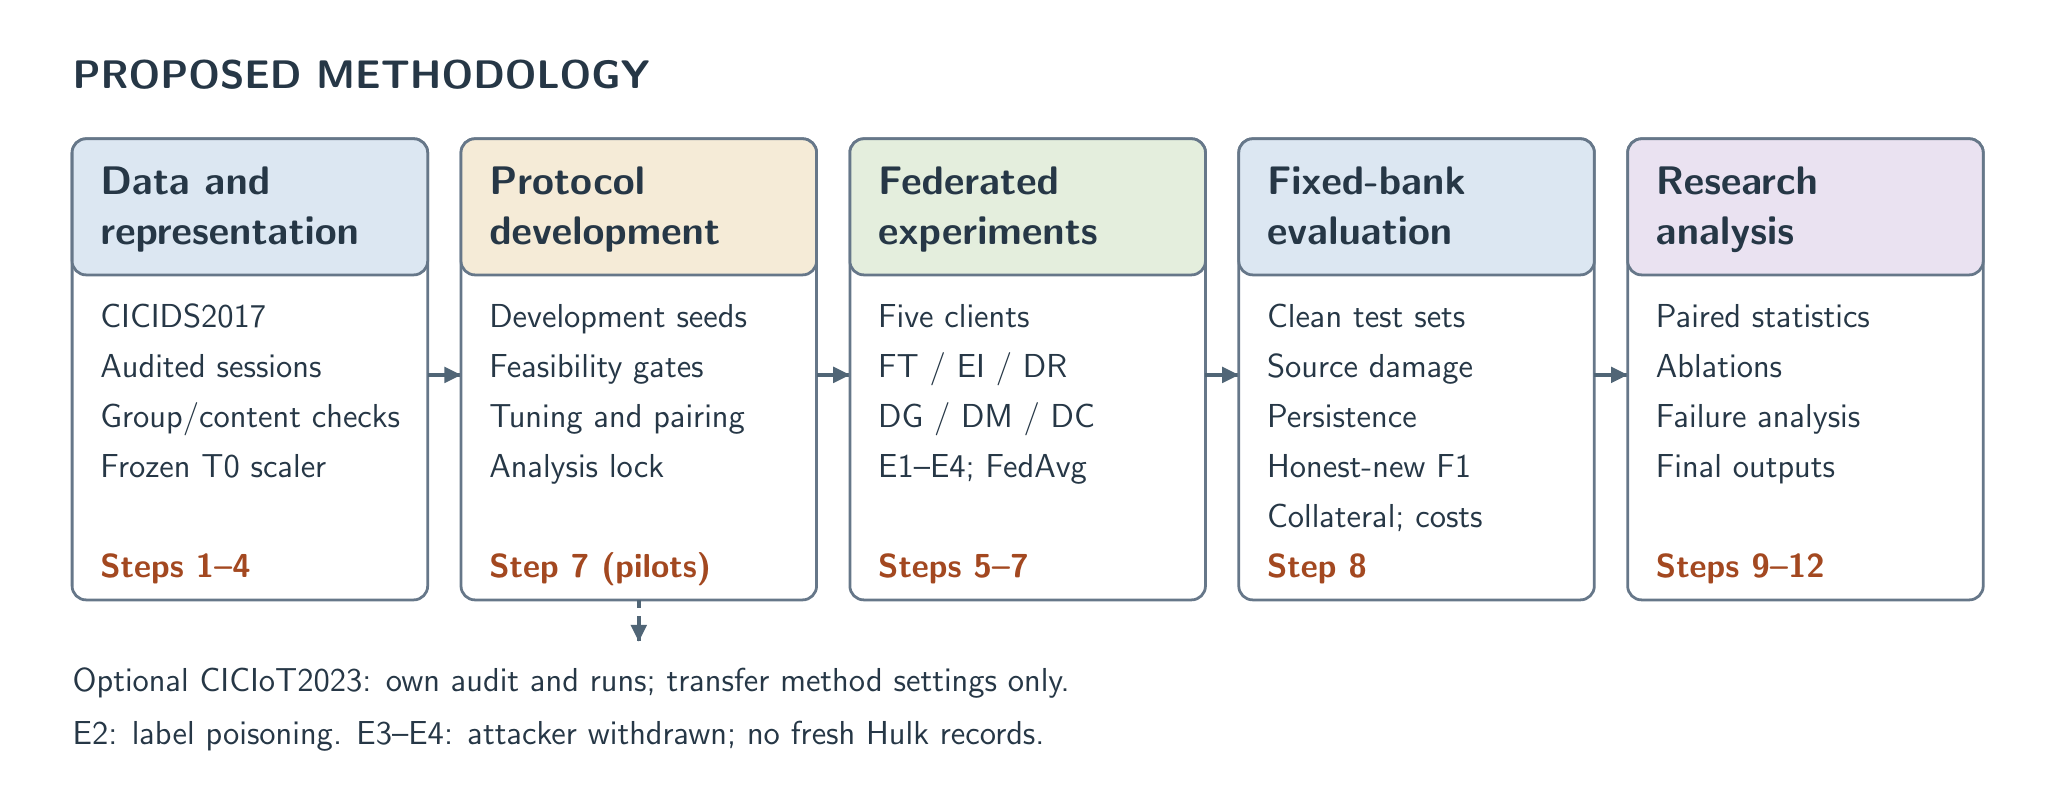
\begin{tikzpicture}[x=1bp,y=-1bp]
\path[use as bounding box] (0,0) rectangle (720,265);
\node[anchor=base west,inner sep=0,text={rgb,255:red,38;green,55;blue,70},font=\sffamily\bfseries\fontsize{15}{17.25}\selectfont] at (16,22) {PROPOSED METHODOLOGY};
\path[draw={rgb,255:red,102;green,119;blue,137},fill={rgb,255:red,255;green,255;blue,255},line width=1bp,rounded corners=5bp] (16,40) rectangle (144,206);
\path[draw={rgb,255:red,102;green,119;blue,137},fill={rgb,255:red,220;green,231;blue,242},line width=1bp,rounded corners=5bp] (16,40) rectangle (144,89);
\node[anchor=base west,inner sep=0,text={rgb,255:red,38;green,55;blue,70},font=\sffamily\bfseries\fontsize{15}{17.25}\selectfont] at (26,60) {Data and};
\node[anchor=base west,inner sep=0,text={rgb,255:red,38;green,55;blue,70},font=\sffamily\bfseries\fontsize{15}{17.25}\selectfont] at (26,78) {representation};
\node[anchor=base west,inner sep=0,text={rgb,255:red,38;green,55;blue,70},font=\sffamily\fontsize{12}{13.8}\selectfont] at (26,108) {CICIDS2017};
\node[anchor=base west,inner sep=0,text={rgb,255:red,38;green,55;blue,70},font=\sffamily\fontsize{12}{13.8}\selectfont] at (26,126) {Audited sessions};
\node[anchor=base west,inner sep=0,text={rgb,255:red,38;green,55;blue,70},font=\sffamily\fontsize{12}{13.8}\selectfont] at (26,144) {Group/content checks};
\node[anchor=base west,inner sep=0,text={rgb,255:red,38;green,55;blue,70},font=\sffamily\fontsize{12}{13.8}\selectfont] at (26,162) {Frozen T0 scaler};
\node[anchor=base west,inner sep=0,text={rgb,255:red,163;green,72;blue,32},font=\sffamily\bfseries\fontsize{12}{13.8}\selectfont] at (26,198) {Steps 1--4};
\path[draw={rgb,255:red,80;green,101;blue,118},line width=1.4bp] (144,125) -- (156,125);
\path[fill={rgb,255:red,80;green,101;blue,118}] (156.000,125.000) -- (150.000,122.000) -- (150.000,128.000) -- cycle;
\path[draw={rgb,255:red,102;green,119;blue,137},fill={rgb,255:red,255;green,255;blue,255},line width=1bp,rounded corners=5bp] (156,40) rectangle (284,206);
\path[draw={rgb,255:red,102;green,119;blue,137},fill={rgb,255:red,245;green,235;blue,215},line width=1bp,rounded corners=5bp] (156,40) rectangle (284,89);
\node[anchor=base west,inner sep=0,text={rgb,255:red,38;green,55;blue,70},font=\sffamily\bfseries\fontsize{15}{17.25}\selectfont] at (166,60) {Protocol};
\node[anchor=base west,inner sep=0,text={rgb,255:red,38;green,55;blue,70},font=\sffamily\bfseries\fontsize{15}{17.25}\selectfont] at (166,78) {development};
\node[anchor=base west,inner sep=0,text={rgb,255:red,38;green,55;blue,70},font=\sffamily\fontsize{12}{13.8}\selectfont] at (166,108) {Development seeds};
\node[anchor=base west,inner sep=0,text={rgb,255:red,38;green,55;blue,70},font=\sffamily\fontsize{12}{13.8}\selectfont] at (166,126) {Feasibility gates};
\node[anchor=base west,inner sep=0,text={rgb,255:red,38;green,55;blue,70},font=\sffamily\fontsize{12}{13.8}\selectfont] at (166,144) {Tuning and pairing};
\node[anchor=base west,inner sep=0,text={rgb,255:red,38;green,55;blue,70},font=\sffamily\fontsize{12}{13.8}\selectfont] at (166,162) {Analysis lock};
\node[anchor=base west,inner sep=0,text={rgb,255:red,163;green,72;blue,32},font=\sffamily\bfseries\fontsize{12}{13.8}\selectfont] at (166,198) {Step 7 (pilots)};
\path[draw={rgb,255:red,80;green,101;blue,118},line width=1.4bp] (284,125) -- (296,125);
\path[fill={rgb,255:red,80;green,101;blue,118}] (296.000,125.000) -- (290.000,122.000) -- (290.000,128.000) -- cycle;
\path[draw={rgb,255:red,102;green,119;blue,137},fill={rgb,255:red,255;green,255;blue,255},line width=1bp,rounded corners=5bp] (296,40) rectangle (424,206);
\path[draw={rgb,255:red,102;green,119;blue,137},fill={rgb,255:red,228;green,238;blue,221},line width=1bp,rounded corners=5bp] (296,40) rectangle (424,89);
\node[anchor=base west,inner sep=0,text={rgb,255:red,38;green,55;blue,70},font=\sffamily\bfseries\fontsize{15}{17.25}\selectfont] at (306,60) {Federated};
\node[anchor=base west,inner sep=0,text={rgb,255:red,38;green,55;blue,70},font=\sffamily\bfseries\fontsize{15}{17.25}\selectfont] at (306,78) {experiments};
\node[anchor=base west,inner sep=0,text={rgb,255:red,38;green,55;blue,70},font=\sffamily\fontsize{12}{13.8}\selectfont] at (306,108) {Five clients};
\node[anchor=base west,inner sep=0,text={rgb,255:red,38;green,55;blue,70},font=\sffamily\fontsize{12}{13.8}\selectfont] at (306,126) {FT / EI / DR};
\node[anchor=base west,inner sep=0,text={rgb,255:red,38;green,55;blue,70},font=\sffamily\fontsize{12}{13.8}\selectfont] at (306,144) {DG / DM / DC};
\node[anchor=base west,inner sep=0,text={rgb,255:red,38;green,55;blue,70},font=\sffamily\fontsize{12}{13.8}\selectfont] at (306,162) {E1--E4; FedAvg};
\node[anchor=base west,inner sep=0,text={rgb,255:red,163;green,72;blue,32},font=\sffamily\bfseries\fontsize{12}{13.8}\selectfont] at (306,198) {Steps 5--7};
\path[draw={rgb,255:red,80;green,101;blue,118},line width=1.4bp] (424,125) -- (436,125);
\path[fill={rgb,255:red,80;green,101;blue,118}] (436.000,125.000) -- (430.000,122.000) -- (430.000,128.000) -- cycle;
\path[draw={rgb,255:red,102;green,119;blue,137},fill={rgb,255:red,255;green,255;blue,255},line width=1bp,rounded corners=5bp] (436,40) rectangle (564,206);
\path[draw={rgb,255:red,102;green,119;blue,137},fill={rgb,255:red,220;green,231;blue,242},line width=1bp,rounded corners=5bp] (436,40) rectangle (564,89);
\node[anchor=base west,inner sep=0,text={rgb,255:red,38;green,55;blue,70},font=\sffamily\bfseries\fontsize{15}{17.25}\selectfont] at (446,60) {Fixed-bank};
\node[anchor=base west,inner sep=0,text={rgb,255:red,38;green,55;blue,70},font=\sffamily\bfseries\fontsize{15}{17.25}\selectfont] at (446,78) {evaluation};
\node[anchor=base west,inner sep=0,text={rgb,255:red,38;green,55;blue,70},font=\sffamily\fontsize{12}{13.8}\selectfont] at (446,108) {Clean test sets};
\node[anchor=base west,inner sep=0,text={rgb,255:red,38;green,55;blue,70},font=\sffamily\fontsize{12}{13.8}\selectfont] at (446,126) {Source damage};
\node[anchor=base west,inner sep=0,text={rgb,255:red,38;green,55;blue,70},font=\sffamily\fontsize{12}{13.8}\selectfont] at (446,144) {Persistence};
\node[anchor=base west,inner sep=0,text={rgb,255:red,38;green,55;blue,70},font=\sffamily\fontsize{12}{13.8}\selectfont] at (446,162) {Honest-new F1};
\node[anchor=base west,inner sep=0,text={rgb,255:red,38;green,55;blue,70},font=\sffamily\fontsize{12}{13.8}\selectfont] at (446,180) {Collateral; costs};
\node[anchor=base west,inner sep=0,text={rgb,255:red,163;green,72;blue,32},font=\sffamily\bfseries\fontsize{12}{13.8}\selectfont] at (446,198) {Step 8};
\path[draw={rgb,255:red,80;green,101;blue,118},line width=1.4bp] (564,125) -- (576,125);
\path[fill={rgb,255:red,80;green,101;blue,118}] (576.000,125.000) -- (570.000,122.000) -- (570.000,128.000) -- cycle;
\path[draw={rgb,255:red,102;green,119;blue,137},fill={rgb,255:red,255;green,255;blue,255},line width=1bp,rounded corners=5bp] (576,40) rectangle (704,206);
\path[draw={rgb,255:red,102;green,119;blue,137},fill={rgb,255:red,234;green,226;blue,241},line width=1bp,rounded corners=5bp] (576,40) rectangle (704,89);
\node[anchor=base west,inner sep=0,text={rgb,255:red,38;green,55;blue,70},font=\sffamily\bfseries\fontsize{15}{17.25}\selectfont] at (586,60) {Research};
\node[anchor=base west,inner sep=0,text={rgb,255:red,38;green,55;blue,70},font=\sffamily\bfseries\fontsize{15}{17.25}\selectfont] at (586,78) {analysis};
\node[anchor=base west,inner sep=0,text={rgb,255:red,38;green,55;blue,70},font=\sffamily\fontsize{12}{13.8}\selectfont] at (586,108) {Paired statistics};
\node[anchor=base west,inner sep=0,text={rgb,255:red,38;green,55;blue,70},font=\sffamily\fontsize{12}{13.8}\selectfont] at (586,126) {Ablations};
\node[anchor=base west,inner sep=0,text={rgb,255:red,38;green,55;blue,70},font=\sffamily\fontsize{12}{13.8}\selectfont] at (586,144) {Failure analysis};
\node[anchor=base west,inner sep=0,text={rgb,255:red,38;green,55;blue,70},font=\sffamily\fontsize{12}{13.8}\selectfont] at (586,162) {Final outputs};
\node[anchor=base west,inner sep=0,text={rgb,255:red,163;green,72;blue,32},font=\sffamily\bfseries\fontsize{12}{13.8}\selectfont] at (586,198) {Steps 9--12};
\path[draw={rgb,255:red,80;green,101;blue,118},line width=1.4bp,dashed] (220,206) -- (220,221);
\path[fill={rgb,255:red,80;green,101;blue,118}] (220,221) -- (223,215) -- (217,215) -- cycle;
\node[anchor=base west,inner sep=0,text={rgb,255:red,38;green,55;blue,70},font=\sffamily\fontsize{12}{13.8}\selectfont] at (16,239) {Optional CICIoT2023: own audit and runs; transfer method settings only.};
\node[anchor=base west,inner sep=0,text={rgb,255:red,38;green,55;blue,70},font=\sffamily\fontsize{12}{13.8}\selectfont] at (16,258) {E2: label poisoning. E3--E4: attacker withdrawn; no fresh Hulk records.};
\end{tikzpicture}
}
\caption{Methodology overview. The orange labels show which of the twelve methodology steps each phase covers. Solid arrows pass audited data, locked settings, trained models and predictions forward; the dashed branch transfers only method settings to the separate exploratory CICIoT2023 study.}
\label{fig:methodology}
\end{figure}

\begin{figure}[H]
\centering
\resizebox{\linewidth}{!}{%
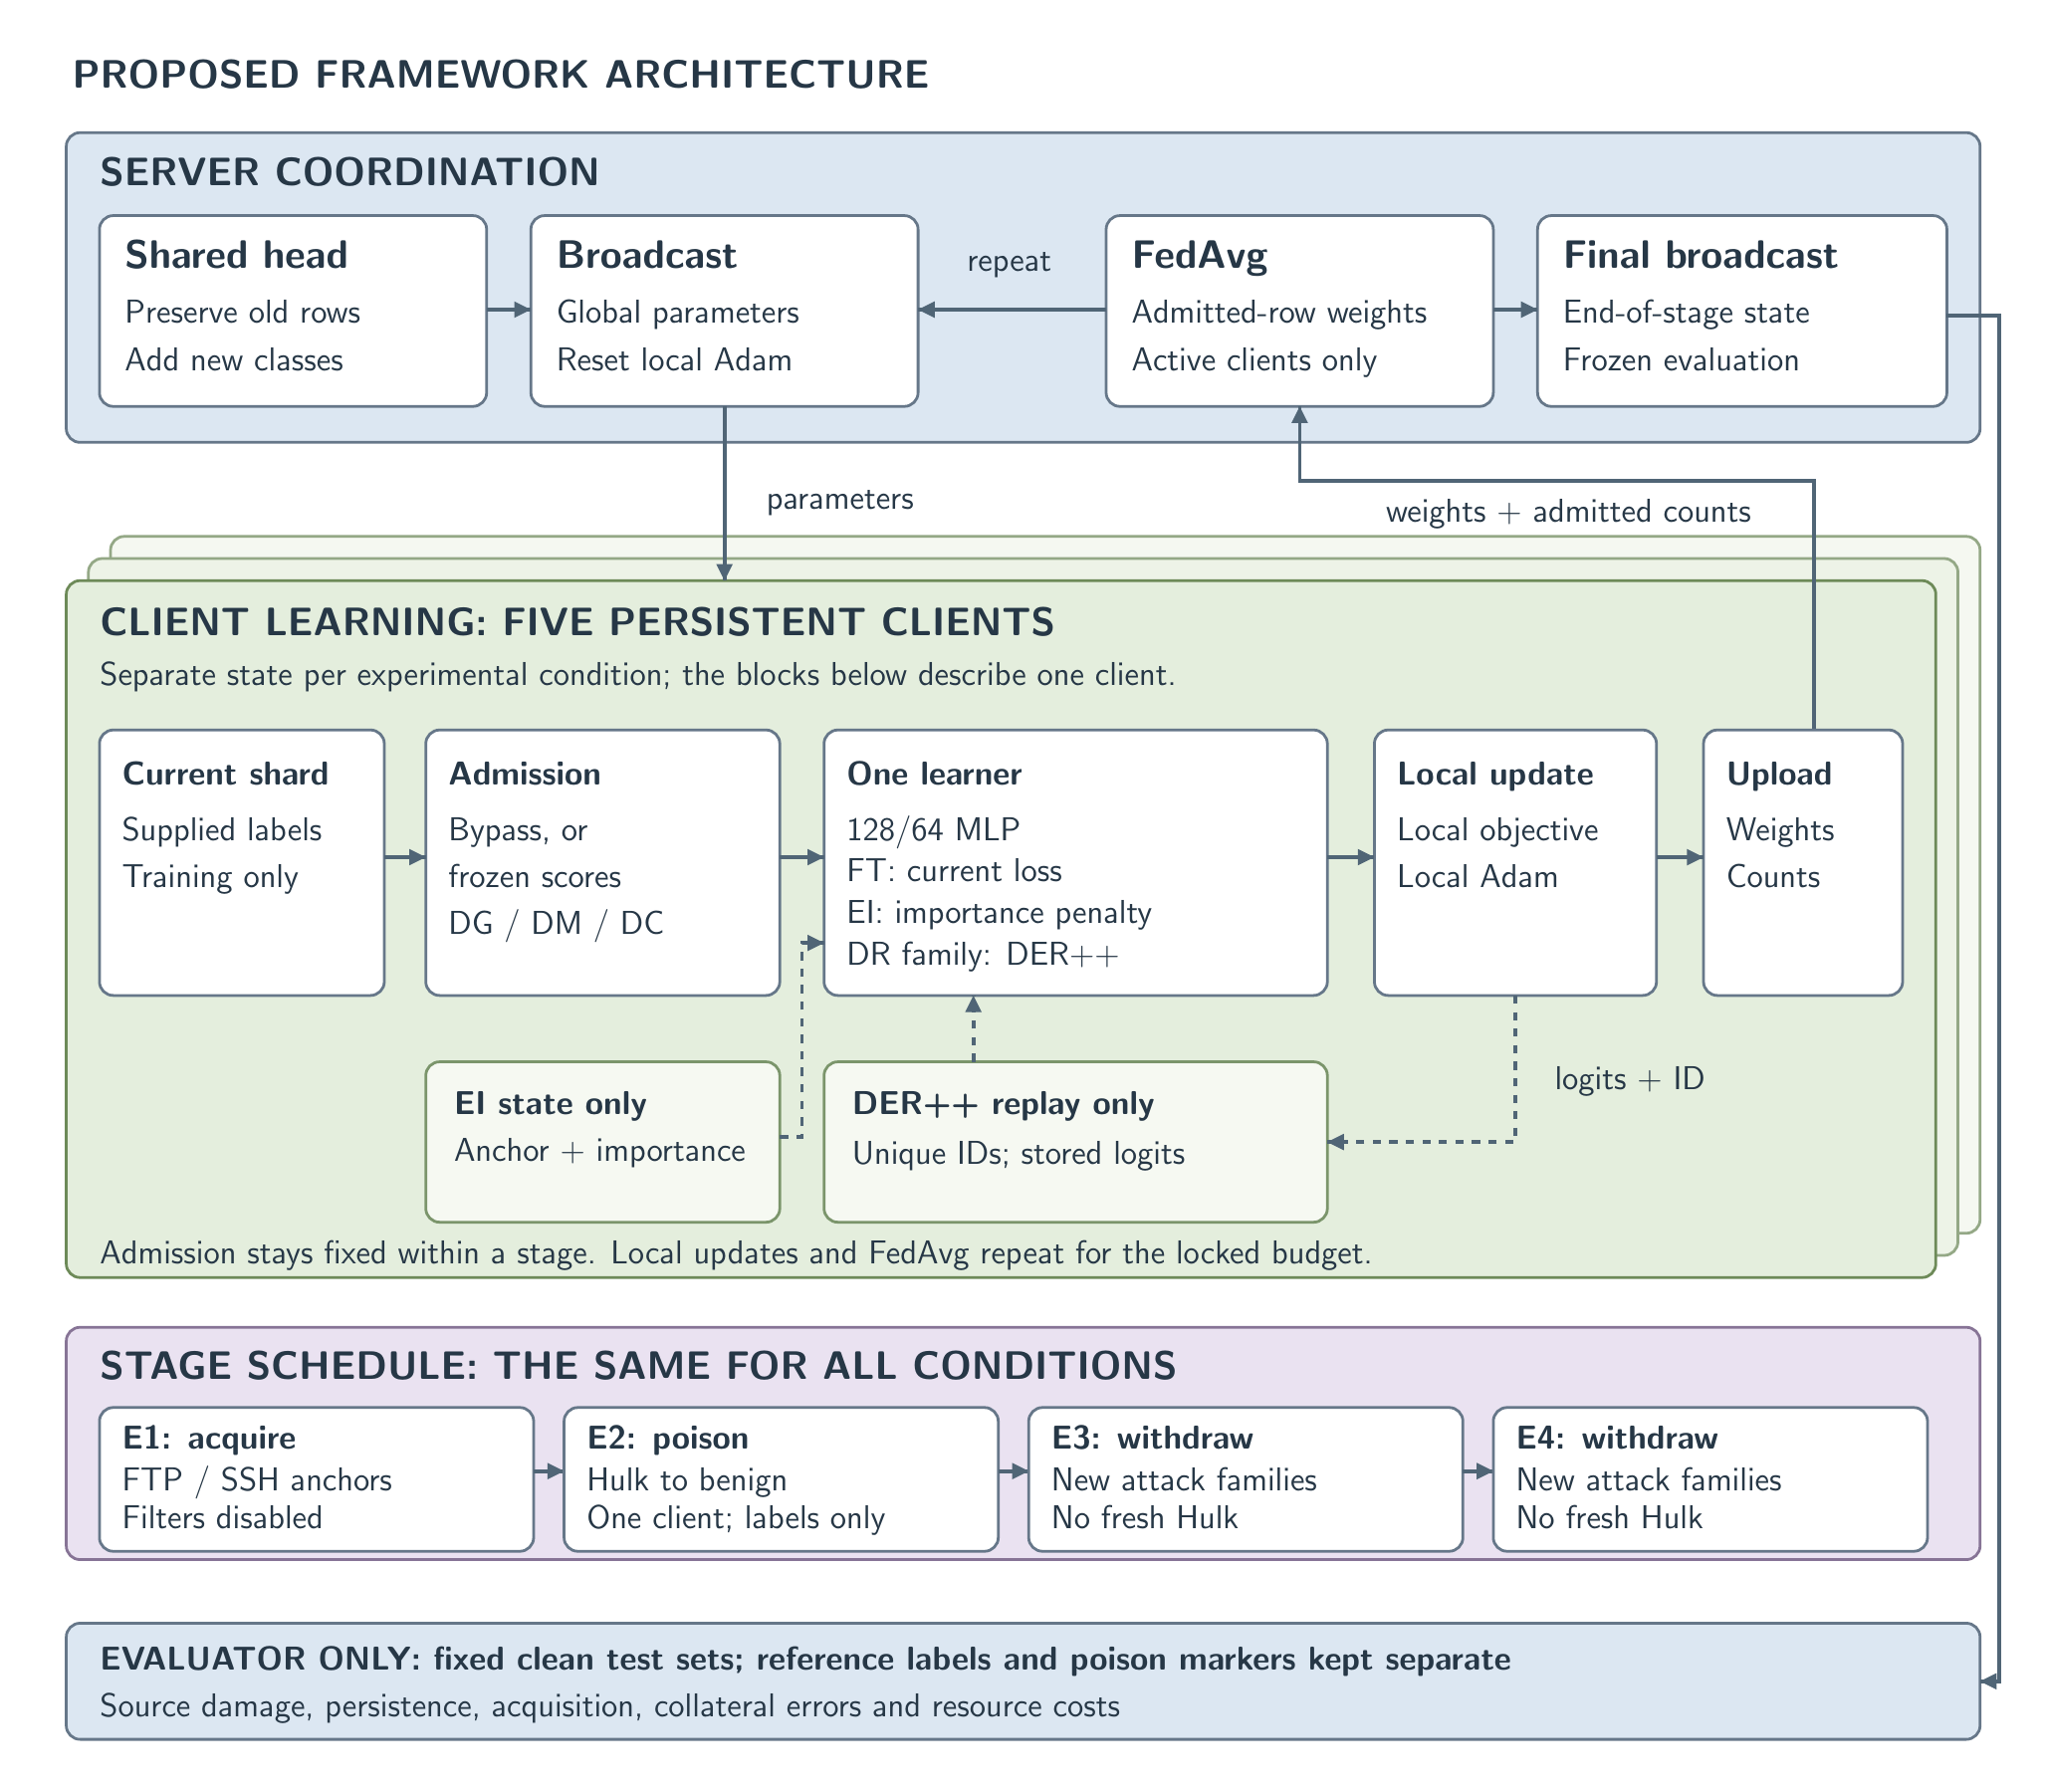
\begin{tikzpicture}[x=1bp,y=-1bp]
\path[use as bounding box] (0,0) rectangle (720,628);
\node[anchor=base west,inner sep=0,text={rgb,255:red,38;green,55;blue,70},font=\sffamily\bfseries\fontsize{15}{17.25}\selectfont] at (16,22) {PROPOSED FRAMEWORK ARCHITECTURE};
\path[draw={rgb,255:red,102;green,119;blue,137},fill={rgb,255:red,220;green,231;blue,242},line width=1bp,rounded corners=5bp] (14,38) rectangle (706,150);
\node[anchor=base west,inner sep=0,text={rgb,255:red,38;green,55;blue,70},font=\sffamily\bfseries\fontsize{15}{17.25}\selectfont] at (26,57) {SERVER COORDINATION};
\path[draw={rgb,255:red,102;green,119;blue,137},fill={rgb,255:red,255;green,255;blue,255},line width=1bp,rounded corners=5bp] (26,68) rectangle (166,137);
\node[anchor=base west,inner sep=0,text={rgb,255:red,38;green,55;blue,70},font=\sffamily\bfseries\fontsize{14}{16.1}\selectfont] at (35,87) {Shared head};
\node[anchor=base west,inner sep=0,text={rgb,255:red,38;green,55;blue,70},font=\sffamily\fontsize{12}{13.8}\selectfont] at (35,107) {Preserve old rows};
\node[anchor=base west,inner sep=0,text={rgb,255:red,38;green,55;blue,70},font=\sffamily\fontsize{12}{13.8}\selectfont] at (35,124) {Add new classes};
\path[draw={rgb,255:red,102;green,119;blue,137},fill={rgb,255:red,255;green,255;blue,255},line width=1bp,rounded corners=5bp] (182,68) rectangle (322,137);
\node[anchor=base west,inner sep=0,text={rgb,255:red,38;green,55;blue,70},font=\sffamily\bfseries\fontsize{14}{16.1}\selectfont] at (191,87) {Broadcast};
\node[anchor=base west,inner sep=0,text={rgb,255:red,38;green,55;blue,70},font=\sffamily\fontsize{12}{13.8}\selectfont] at (191,107) {Global parameters};
\node[anchor=base west,inner sep=0,text={rgb,255:red,38;green,55;blue,70},font=\sffamily\fontsize{12}{13.8}\selectfont] at (191,124) {Reset local Adam};
\path[draw={rgb,255:red,102;green,119;blue,137},fill={rgb,255:red,255;green,255;blue,255},line width=1bp,rounded corners=5bp] (390,68) rectangle (530,137);
\node[anchor=base west,inner sep=0,text={rgb,255:red,38;green,55;blue,70},font=\sffamily\bfseries\fontsize{14}{16.1}\selectfont] at (399,87) {FedAvg};
\node[anchor=base west,inner sep=0,text={rgb,255:red,38;green,55;blue,70},font=\sffamily\fontsize{12}{13.8}\selectfont] at (399,107) {Admitted-row weights};
\node[anchor=base west,inner sep=0,text={rgb,255:red,38;green,55;blue,70},font=\sffamily\fontsize{12}{13.8}\selectfont] at (399,124) {Active clients only};
\path[draw={rgb,255:red,102;green,119;blue,137},fill={rgb,255:red,255;green,255;blue,255},line width=1bp,rounded corners=5bp] (546,68) rectangle (694,137);
\node[anchor=base west,inner sep=0,text={rgb,255:red,38;green,55;blue,70},font=\sffamily\bfseries\fontsize{14}{16.1}\selectfont] at (555,87) {Final broadcast};
\node[anchor=base west,inner sep=0,text={rgb,255:red,38;green,55;blue,70},font=\sffamily\fontsize{12}{13.8}\selectfont] at (555,107) {End-of-stage state};
\node[anchor=base west,inner sep=0,text={rgb,255:red,38;green,55;blue,70},font=\sffamily\fontsize{12}{13.8}\selectfont] at (555,124) {Frozen evaluation};
\path[draw={rgb,255:red,80;green,101;blue,118},line width=1.4bp] (166,102) -- (182,102);
\path[fill={rgb,255:red,80;green,101;blue,118}] (182.000,102.000) -- (176.000,99.000) -- (176.000,105.000) -- cycle;
\path[draw={rgb,255:red,80;green,101;blue,118},line width=1.4bp] (530,102) -- (546,102);
\path[fill={rgb,255:red,80;green,101;blue,118}] (546.000,102.000) -- (540.000,99.000) -- (540.000,105.000) -- cycle;
\path[draw={rgb,255:red,80;green,101;blue,118},line width=1.4bp] (390,102) -- (322,102);
\path[fill={rgb,255:red,80;green,101;blue,118}] (322.000,102.000) -- (328.000,105.000) -- (328.000,99.000) -- cycle;
\node[anchor=base,inner sep=0,text={rgb,255:red,38;green,55;blue,70},font=\sffamily\fontsize{12}{13.8}\selectfont] at (355,88) {repeat};
\path[draw={rgb,255:red,148;green,168;blue,134},fill={rgb,255:red,245;green,248;blue,241},line width=1bp,rounded corners=5bp] (30,184) rectangle (706,436);
\path[draw={rgb,255:red,148;green,168;blue,134},fill={rgb,255:red,237;green,243;blue,231},line width=1bp,rounded corners=5bp] (22,192) rectangle (698,444);
\path[draw={rgb,255:red,109;green,138;blue,88},fill={rgb,255:red,228;green,238;blue,221},line width=1bp,rounded corners=5bp] (14,200) rectangle (690,452);
\node[anchor=base west,inner sep=0,text={rgb,255:red,38;green,55;blue,70},font=\sffamily\bfseries\fontsize{15}{17.25}\selectfont] at (26,220) {CLIENT LEARNING: FIVE PERSISTENT CLIENTS};
\node[anchor=base west,inner sep=0,text={rgb,255:red,38;green,55;blue,70},font=\sffamily\fontsize{12}{13.8}\selectfont] at (26,238) {Separate state per experimental condition; the blocks below describe one client.};
\path[draw={rgb,255:red,80;green,101;blue,118},line width=1.4bp] (252,137) -- (252,200);
\path[fill={rgb,255:red,80;green,101;blue,118}] (252.000,200.000) -- (255.000,194.000) -- (249.000,194.000) -- cycle;
\node[anchor=base west,inner sep=0,text={rgb,255:red,38;green,55;blue,70},font=\sffamily\fontsize{12}{13.8}\selectfont] at (267,174) {parameters};
\path[draw={rgb,255:red,80;green,101;blue,118},line width=1.4bp] (646,254) -- (646,164) -- (460,164) -- (460,137);
\path[fill={rgb,255:red,80;green,101;blue,118}] (460.000,137.000) -- (457.000,143.000) -- (463.000,143.000) -- cycle;
\node[anchor=base west,inner sep=0,text={rgb,255:red,38;green,55;blue,70},font=\sffamily\fontsize{12}{13.8}\selectfont] at (491,179) {weights + admitted counts};
\path[draw={rgb,255:red,102;green,119;blue,137},fill={rgb,255:red,255;green,255;blue,255},line width=1bp,rounded corners=5bp] (26,254) rectangle (129,350);
\node[anchor=base west,inner sep=0,text={rgb,255:red,38;green,55;blue,70},font=\sffamily\bfseries\fontsize{13}{14.95}\selectfont] at (34,274) {Current shard};
\node[anchor=base west,inner sep=0,text={rgb,255:red,38;green,55;blue,70},font=\sffamily\fontsize{12}{13.8}\selectfont] at (34,294) {Supplied labels};
\node[anchor=base west,inner sep=0,text={rgb,255:red,38;green,55;blue,70},font=\sffamily\fontsize{12}{13.8}\selectfont] at (34,311) {Training only};
\path[draw={rgb,255:red,102;green,119;blue,137},fill={rgb,255:red,255;green,255;blue,255},line width=1bp,rounded corners=5bp] (144,254) rectangle (272,350);
\node[anchor=base west,inner sep=0,text={rgb,255:red,38;green,55;blue,70},font=\sffamily\bfseries\fontsize{13}{14.95}\selectfont] at (152,274) {Admission};
\node[anchor=base west,inner sep=0,text={rgb,255:red,38;green,55;blue,70},font=\sffamily\fontsize{12}{13.8}\selectfont] at (152,294) {Bypass, or};
\node[anchor=base west,inner sep=0,text={rgb,255:red,38;green,55;blue,70},font=\sffamily\fontsize{12}{13.8}\selectfont] at (152,311) {frozen scores};
\node[anchor=base west,inner sep=0,text={rgb,255:red,38;green,55;blue,70},font=\sffamily\fontsize{12}{13.8}\selectfont] at (152,328) {DG / DM / DC};
\path[draw={rgb,255:red,102;green,119;blue,137},fill={rgb,255:red,255;green,255;blue,255},line width=1bp,rounded corners=5bp] (288,254) rectangle (470,350);
\node[anchor=base west,inner sep=0,text={rgb,255:red,38;green,55;blue,70},font=\sffamily\bfseries\fontsize{13}{14.95}\selectfont] at (296,274) {One learner};
\node[anchor=base west,inner sep=0,text={rgb,255:red,38;green,55;blue,70},font=\sffamily\fontsize{12}{13.8}\selectfont] at (296,294) {128/64 MLP};
\node[anchor=base west,inner sep=0,text={rgb,255:red,38;green,55;blue,70},font=\sffamily\fontsize{12}{13.8}\selectfont] at (296,309) {FT: current loss};
\node[anchor=base west,inner sep=0,text={rgb,255:red,38;green,55;blue,70},font=\sffamily\fontsize{12}{13.8}\selectfont] at (296,324) {EI: importance penalty};
\node[anchor=base west,inner sep=0,text={rgb,255:red,38;green,55;blue,70},font=\sffamily\fontsize{12}{13.8}\selectfont] at (296,339) {DR family: DER++};
\path[draw={rgb,255:red,102;green,119;blue,137},fill={rgb,255:red,255;green,255;blue,255},line width=1bp,rounded corners=5bp] (487,254) rectangle (589,350);
\node[anchor=base west,inner sep=0,text={rgb,255:red,38;green,55;blue,70},font=\sffamily\bfseries\fontsize{13}{14.95}\selectfont] at (495,274) {Local update};
\node[anchor=base west,inner sep=0,text={rgb,255:red,38;green,55;blue,70},font=\sffamily\fontsize{12}{13.8}\selectfont] at (495,294) {Local objective};
\node[anchor=base west,inner sep=0,text={rgb,255:red,38;green,55;blue,70},font=\sffamily\fontsize{12}{13.8}\selectfont] at (495,311) {Local Adam};
\path[draw={rgb,255:red,102;green,119;blue,137},fill={rgb,255:red,255;green,255;blue,255},line width=1bp,rounded corners=5bp] (606,254) rectangle (678,350);
\node[anchor=base west,inner sep=0,text={rgb,255:red,38;green,55;blue,70},font=\sffamily\bfseries\fontsize{13}{14.95}\selectfont] at (614,274) {Upload};
\node[anchor=base west,inner sep=0,text={rgb,255:red,38;green,55;blue,70},font=\sffamily\fontsize{12}{13.8}\selectfont] at (614,294) {Weights};
\node[anchor=base west,inner sep=0,text={rgb,255:red,38;green,55;blue,70},font=\sffamily\fontsize{12}{13.8}\selectfont] at (614,311) {Counts};
\path[draw={rgb,255:red,80;green,101;blue,118},line width=1.4bp] (129,300) -- (144,300);
\path[fill={rgb,255:red,80;green,101;blue,118}] (144.000,300.000) -- (138.000,297.000) -- (138.000,303.000) -- cycle;
\path[draw={rgb,255:red,80;green,101;blue,118},line width=1.4bp] (272,300) -- (288,300);
\path[fill={rgb,255:red,80;green,101;blue,118}] (288.000,300.000) -- (282.000,297.000) -- (282.000,303.000) -- cycle;
\path[draw={rgb,255:red,80;green,101;blue,118},line width=1.4bp] (470,300) -- (487,300);
\path[fill={rgb,255:red,80;green,101;blue,118}] (487.000,300.000) -- (481.000,297.000) -- (481.000,303.000) -- cycle;
\path[draw={rgb,255:red,80;green,101;blue,118},line width=1.4bp] (589,300) -- (606,300);
\path[fill={rgb,255:red,80;green,101;blue,118}] (606.000,300.000) -- (600.000,297.000) -- (600.000,303.000) -- cycle;
\path[draw={rgb,255:red,123;green,149;blue,107},fill={rgb,255:red,246;green,249;blue,242},line width=1bp,rounded corners=5bp] (144,374) rectangle (272,432);
\node[anchor=base west,inner sep=0,text={rgb,255:red,38;green,55;blue,70},font=\sffamily\bfseries\fontsize{13}{14.95}\selectfont] at (154,393) {EI state only};
\node[anchor=base west,inner sep=0,text={rgb,255:red,38;green,55;blue,70},font=\sffamily\fontsize{12}{13.8}\selectfont] at (154,410) {Anchor + importance};
\path[draw={rgb,255:red,80;green,101;blue,118},line width=1.4bp,dashed] (272,401) -- (280,401) -- (280,331) -- (288,331);
\path[fill={rgb,255:red,80;green,101;blue,118}] (288.000,331.000) -- (282.000,328.000) -- (282.000,334.000) -- cycle;
\path[draw={rgb,255:red,123;green,149;blue,107},fill={rgb,255:red,246;green,249;blue,242},line width=1bp,rounded corners=5bp] (288,374) rectangle (470,432);
\node[anchor=base west,inner sep=0,text={rgb,255:red,38;green,55;blue,70},font=\sffamily\bfseries\fontsize{13}{14.95}\selectfont] at (298,393) {DER++ replay only};
\node[anchor=base west,inner sep=0,text={rgb,255:red,38;green,55;blue,70},font=\sffamily\fontsize{12}{13.8}\selectfont] at (298,411) {Unique IDs; stored logits};
\path[draw={rgb,255:red,80;green,101;blue,118},line width=1.4bp,dashed] (342,374) -- (342,350);
\path[fill={rgb,255:red,80;green,101;blue,118}] (342.000,350.000) -- (339.000,356.000) -- (345.000,356.000) -- cycle;
\path[draw={rgb,255:red,80;green,101;blue,118},line width=1.4bp,dashed] (538,350) -- (538,403) -- (470,403);
\path[fill={rgb,255:red,80;green,101;blue,118}] (470.000,403.000) -- (476.000,406.000) -- (476.000,400.000) -- cycle;
\node[anchor=base west,inner sep=0,text={rgb,255:red,38;green,55;blue,70},font=\sffamily\fontsize{12}{13.8}\selectfont] at (552,384) {logits + ID};
\node[anchor=base west,inner sep=0,text={rgb,255:red,38;green,55;blue,70},font=\sffamily\fontsize{12}{13.8}\selectfont] at (26,447) {Admission stays fixed within a stage. Local updates and FedAvg repeat for the locked budget.};
\path[draw={rgb,255:red,135;green,116;blue,150},fill={rgb,255:red,234;green,226;blue,241},line width=1bp,rounded corners=5bp] (14,470) rectangle (706,554);
\node[anchor=base west,inner sep=0,text={rgb,255:red,38;green,55;blue,70},font=\sffamily\bfseries\fontsize{15}{17.25}\selectfont] at (26,489) {STAGE SCHEDULE: THE SAME FOR ALL CONDITIONS};
\path[draw={rgb,255:red,102;green,119;blue,137},fill={rgb,255:red,255;green,255;blue,255},line width=1bp,rounded corners=5bp] (26,499) rectangle (183,551);
\node[anchor=base west,inner sep=0,text={rgb,255:red,38;green,55;blue,70},font=\sffamily\bfseries\fontsize{13}{14.95}\selectfont] at (34,514) {E1: acquire};
\node[anchor=base west,inner sep=0,text={rgb,255:red,38;green,55;blue,70},font=\sffamily\fontsize{12}{13.8}\selectfont] at (34,529) {FTP / SSH anchors};
\node[anchor=base west,inner sep=0,text={rgb,255:red,38;green,55;blue,70},font=\sffamily\fontsize{12}{13.8}\selectfont] at (34,543) {Filters disabled};
\path[draw={rgb,255:red,80;green,101;blue,118},line width=1.4bp] (183,522) -- (194,522);
\path[fill={rgb,255:red,80;green,101;blue,118}] (194.000,522.000) -- (188.000,519.000) -- (188.000,525.000) -- cycle;
\path[draw={rgb,255:red,102;green,119;blue,137},fill={rgb,255:red,255;green,255;blue,255},line width=1bp,rounded corners=5bp] (194,499) rectangle (351,551);
\node[anchor=base west,inner sep=0,text={rgb,255:red,38;green,55;blue,70},font=\sffamily\bfseries\fontsize{13}{14.95}\selectfont] at (202,514) {E2: poison};
\node[anchor=base west,inner sep=0,text={rgb,255:red,38;green,55;blue,70},font=\sffamily\fontsize{12}{13.8}\selectfont] at (202,529) {Hulk to benign};
\node[anchor=base west,inner sep=0,text={rgb,255:red,38;green,55;blue,70},font=\sffamily\fontsize{12}{13.8}\selectfont] at (202,543) {One client; labels only};
\path[draw={rgb,255:red,80;green,101;blue,118},line width=1.4bp] (351,522) -- (362,522);
\path[fill={rgb,255:red,80;green,101;blue,118}] (362.000,522.000) -- (356.000,519.000) -- (356.000,525.000) -- cycle;
\path[draw={rgb,255:red,102;green,119;blue,137},fill={rgb,255:red,255;green,255;blue,255},line width=1bp,rounded corners=5bp] (362,499) rectangle (519,551);
\node[anchor=base west,inner sep=0,text={rgb,255:red,38;green,55;blue,70},font=\sffamily\bfseries\fontsize{13}{14.95}\selectfont] at (370,514) {E3: withdraw};
\node[anchor=base west,inner sep=0,text={rgb,255:red,38;green,55;blue,70},font=\sffamily\fontsize{12}{13.8}\selectfont] at (370,529) {New attack families};
\node[anchor=base west,inner sep=0,text={rgb,255:red,38;green,55;blue,70},font=\sffamily\fontsize{12}{13.8}\selectfont] at (370,543) {No fresh Hulk};
\path[draw={rgb,255:red,80;green,101;blue,118},line width=1.4bp] (519,522) -- (530,522);
\path[fill={rgb,255:red,80;green,101;blue,118}] (530.000,522.000) -- (524.000,519.000) -- (524.000,525.000) -- cycle;
\path[draw={rgb,255:red,102;green,119;blue,137},fill={rgb,255:red,255;green,255;blue,255},line width=1bp,rounded corners=5bp] (530,499) rectangle (687,551);
\node[anchor=base west,inner sep=0,text={rgb,255:red,38;green,55;blue,70},font=\sffamily\bfseries\fontsize{13}{14.95}\selectfont] at (538,514) {E4: withdraw};
\node[anchor=base west,inner sep=0,text={rgb,255:red,38;green,55;blue,70},font=\sffamily\fontsize{12}{13.8}\selectfont] at (538,529) {New attack families};
\node[anchor=base west,inner sep=0,text={rgb,255:red,38;green,55;blue,70},font=\sffamily\fontsize{12}{13.8}\selectfont] at (538,543) {No fresh Hulk};
\path[draw={rgb,255:red,102;green,119;blue,137},fill={rgb,255:red,220;green,231;blue,242},line width=1bp,rounded corners=5bp] (14,577) rectangle (706,619);
\node[anchor=base west,inner sep=0,text={rgb,255:red,38;green,55;blue,70},font=\sffamily\bfseries\fontsize{13}{14.95}\selectfont] at (26,594) {EVALUATOR ONLY: fixed clean test sets; reference labels and poison markers kept separate};
\node[anchor=base west,inner sep=0,text={rgb,255:red,38;green,55;blue,70},font=\sffamily\fontsize{12}{13.8}\selectfont] at (26,611) {Source damage, persistence, acquisition, collateral errors and resource costs};
\path[draw={rgb,255:red,80;green,101;blue,118},line width=1.4bp] (694,104) -- (713,104) -- (713,598) -- (706,598);
\path[fill={rgb,255:red,80;green,101;blue,118}] (706.000,598.000) -- (712.000,601.000) -- (712.000,595.000) -- cycle;
\end{tikzpicture}
}
\caption{Proposed framework architecture. Server coordination and client learning repeat within each stage. FT/EI/DR are alternative learners; DG/DM/DC are alternative admission rules on DER++. Only EI keeps importance state and only DER++ conditions keep replay memory (dashed links). E2 corrupts training labels at one client only; E3--E4 contain no poison and no fresh Hulk data. The evaluator never influences training or admission.}
\label{fig:framework}
\end{figure}

%=====================================================================
\section{Scope and Threats to Validity}
\textbf{Internal validity.} Operational session grouping, known label defects, duplicate flows and optimiser choices can bias comparisons. Group/content audits and clean-learning gates reduce these risks without proving perfect isolation. A group-stratified split supports a controlled class-arrival simulation, not a claim of globally chronological online generalisation. The admission rule may still keep low-loss poisoned rows; this is a possible finding, not a flaw.

\textbf{External validity.} Clients are simulated by splitting one historical capture, so they do not represent independent organisations (a limitation shared with P5, P7 and P11). CICIoT2023 is a planned, independently audited exploratory check, and CPU timings and update sizes do not measure energy or network delay on real edge devices.

\textbf{Construct validity.} Source recall, persistent error, acquisition and anchor scores measure different things and are reported separately. Withdrawal without fresh Hulk data measures persistence, not recovery after correctly labelled Hulk traffic returns. The attacker controls labels only; a fully compromised client that skips filtering is a stronger, separate threat. Session-separated flows can still share hosts or collection artefacts, so identifier exclusion does not establish cross-site generalisation.

\textbf{Conclusion validity.} Twelve seeds measure training variability with fixed test sets, not variability between captures. Signed-rank tests assume independent seed-level differences with an approximately symmetric distribution. One Holm correction controls the 29 confirmatory tests jointly at 5\% under valid marginal tests; small samples and many contrasts can leave low power. Unadjusted bootstrap intervals describe seed variability only.

%=====================================================================
\appendix
\section{Notation and Data-Isolation Conditions}
\label{app:notation}
\begin{table}[H]
\centering\footnotesize
\caption{Main notation.}
\label{tab:notation}
\begin{tabularx}{\linewidth}{L{4.6cm}Y}
\toprule
Symbol & Meaning\\
\midrule
$k,\ t,\ c,\ i,\ s$ & Client, stage, class, record and seed indices\\
$x_i,\ \widetilde y_i,\ y_i,\ \widehat y_i$ & Features; supplied (possibly poisoned), reference and predicted labels\\
$u_i,\ \sigma_i,\ \tau_i$ & Immutable record ID, session ID and timestamp (metadata only)\\
$\mathcal C_t,\ \mathcal C_t^{\rm new},\ C_t,\ \mathcal U_t$ & Active classes, newly registered classes, active head width, eligible untargeted new families\\
$W,\ b,\ \theta,\ f_{\theta,t}$ & Weights, biases, all parameters, output logits\\
$\mathcal B,\ m,\ z_i,\ \omega_i,\ S_i$ & Replay memory, its capacity (500), stored logits, their width, logit selector\\
$\lambda_E,\ \lambda_z,\ \lambda_y,\ I_{k,a}$ & Loss weights and accumulated parameter importance\\
$n_{k,c,t},\ K_{k,c,t}$ & Rows of class $c$ at client $k$ in stage $t$; admitted quota\\
$\rho,\ Q_{k,2}$ & Poison dose and number of flipped Hulk rows\\
$\mathcal S_{\rm tr/dev/te},\ \mathcal G_{\rm tr/dev/te},\ H_{\rm sha},\ \Psi_0$ & Splits, their sessions, content hash, frozen T0 scaler\\
$\mathrm{ASR},\ H,\ \Delta_{\rm rec},\ A,\ \mathrm{FAR}_B$ & Attack success, persistence, recall change, acquisition, benign false alarms\\
\bottomrule
\end{tabularx}
\end{table}
The hash $H_{\rm sha}$ denotes the set of canonical feature hashes in a set of records. For each pair of distinct splits $a,b\in\{\mathrm{tr},\mathrm{dev},\mathrm{te}\}$,
\begin{equation}
\begin{aligned}
H_{\rm sha}(\mathcal S_a)\cap H_{\rm sha}(\mathcal S_b)&=\varnothing,\\
\mathcal G_a\cap\mathcal G_b&=\varnothing,\\
H_{\rm sha}(T0)\cap H_{\rm sha}(\mathcal S_a)&=\varnothing,\qquad
\mathcal G_{T0}\cap\mathcal G_a=\varnothing.
\end{aligned}
\label{eq:isolation}
\end{equation}
The scaler is $\Psi_0=\operatorname{FitMinMax}(T0)$; it is never refitted. Ownership is disjoint across clients and fresh record IDs are disjoint across stages; replay of a past training record is the intentional exception to fresh-stage use.

\section{Continual-Learning Metric Definitions}
\label{app:metrics}
Let $R_{t,j}$ be accuracy after stage $t$ on the fixed stage-$j$ test cohort (its eligible attack families and its disjoint benign cohort), predicting over all classes currently registered. Later-class predictions on an earlier cohort count as errors. For $T=4$,
\begin{equation}
\begin{aligned}
\mathrm{ACC}_T&=\tfrac1T\sum_{j=1}^{T}R_{T,j},\\
\mathrm{BWT}_T&=\tfrac1{T-1}\sum_{j=1}^{T-1}(R_{T,j}-R_{j,j}),\\
F_T&=\tfrac1{T-1}\sum_{j=1}^{T-1}\left(\max_{\ell=j,\ldots,T}R_{\ell,j}-R_{T,j}\right).
\end{aligned}
\end{equation}
ACC is an equal-stage mean, not pooled sample accuracy. Macro-F1 averages the fixed eligible seen classes on the cumulative bank, including benign; the separate acquisition endpoint excludes Hulk and benign. FAR$_B$ is the fraction of the fixed benign bank assigned any attack label. Report denominator counts and support alongside these scores.

\section{Statistical Details}
\label{app:stats}
The endpoints $H$ and $\Delta_{\rm rec}$ already subtract the matching clean run. Therefore the learner contrast is
\begin{equation}
\mathcal J_s^{\mathsf A,\mathsf B}(\rho;U)
=U_s^{\mathsf A}(\rho)-U_s^{\mathsf B}(\rho),\qquad U\in\{H,\Delta_{\rm rec}\},
\label{eq:interaction}
\end{equation}
without a second baseline subtraction. C1 uses the three learner pairs at three non-zero doses for each of those two endpoints (18 tests). C2 uses DC minus DM in $A$ at all four doses (4), $H$ and $\Delta_{\rm rec}$ at the three non-zero doses (6), and clean E4 FAR$_B$ (1).

For each contrast, compute twelve paired differences $\delta_s$. Drop exact zero differences from signed ranking, average ranks of tied absolute differences, and enumerate all $2^m$ signs on the $m$ non-zero ranked differences for a two-sided signed-rank p-value; all-zero differences give $p=1$ and rank-biserial effect zero. Report $m$ and ties. The rank-biserial effect is $(W_+-W_-)/(W_++W_-)$ for a non-empty rank set. Test validity relies on symmetry of the difference distribution; enumeration does not remove that assumption. An exact paired sign test is an exploratory sensitivity check when symmetry is doubtful.

Holm correction orders all $L=29$ p-values and compares the $h$-th with $0.05/(L-h+1)$, stopping at the first failure \cite{holm}. Whole-seed bootstrap samples preserve the pair:
\begin{equation}
\begin{aligned}
\delta_b^*&=\tfrac1{12}\sum_{\kappa=1}^{12}\delta_{\mathcal I_\kappa},\quad
\mathcal I_\kappa\sim\operatorname{Uniform}\{1,\ldots,12\},\\
\mathrm{CI}_{\rm boot}&=[\operatorname{Quant}_{0.025}(\delta^*),\operatorname{Quant}_{0.975}(\delta^*)].
\end{aligned}
\label{eq:bootstrap}
\end{equation}
These descriptive percentile intervals are neither exact nor adjusted for 29 comparisons. With only twelve seeds, interval coverage and tail estimates can be unstable; interpret them with the raw paired trajectories.

\textbf{Resolution and missingness.} The smallest two-sided p-value for $m$ non-zero pairs is $2/2^m$. The first Holm cutoff is $0.05/29\simeq0.00172$, requiring at least eleven non-zero pairs for that first rejection; later cutoffs can be less strict. This is a resolution calculation, not power. Failed trajectories are repaired and rerun with their complete matched set. If a predeclared endpoint cannot be restored, no zero or favourable replacement is imputed: its confirmatory test is reported unavailable (assigned $p=1$ for the fixed Holm bookkeeping), with a documented protocol deviation. Conclusions remain conditional on this capture, split and threat.

\section{CICIDS2017 Source Files}
\label{app:files}
Numeric features and session metadata are projected together from the eight TrafficLabelling CSVs in \emph{GeneratedLabelledFlows}. The eight MachineLearningCSV files are: \path{Monday-WorkingHours.pcap_ISCX.csv}, \path{Tuesday-WorkingHours.pcap_ISCX.csv}, \path{Wednesday-workingHours.pcap_ISCX.csv}, \path{Thursday-WorkingHours-Morning-WebAttacks.pcap_ISCX.csv}, \path{Thursday-WorkingHours-Afternoon-Infilteration.pcap_ISCX.csv}, \path{Friday-WorkingHours-Morning.pcap_ISCX.csv}, \path{Friday-WorkingHours-Afternoon-PortScan.pcap_ISCX.csv} and \path{Friday-WorkingHours-Afternoon-DDos.pcap_ISCX.csv}.

%=====================================================================
\begin{thebibliography}{99}
\bibitem{phase1} Saneedullah and A. Bilal, \enquote{Continual learning for network security: Phase 1 literature review and research gap identification,} Computer Networks course report, FAST-NUCES, 2026.
\bibitem{ge} J. Ge, Y. Feng, and K. Sakurai, \enquote{A stage-wise framework using class-incremental learning for unknown DoS attack detection,} \emph{Future Internet}, vol. 18, no. 3, Art. 145, 2026. \url{https://doi.org/10.3390/fi18030145}.
\bibitem{wu} Z. Wu, B. He, Z. Si, C. Qiu, X. Liao, and C. Su, \enquote{Communication-efficient federated class-incremental intrusion detection for edge IoT networks,} \emph{Sensors}, vol. 26, no. 14, Art. 4630, 2026. \url{https://doi.org/10.3390/s26144630}.
\bibitem{luo} F. Luo, S. Fan, X. Li, and W. Xu, \enquote{Adaptive feature distillation-based continuous authentication against RF fingerprint drift for power equipment,} \emph{Future Internet}, vol. 18, no. 9, Art. 457, 2026. \url{https://doi.org/10.3390/fi18090457}.
\bibitem{clarivate} Clarivate, \enquote{Journal Citation Reports 2025 release (2024 JIF data),} Jun. 18, 2025. \url{https://clarivate.com/news/clarivate-unveils-the-2025-journal-citation-reports/}.
\bibitem{jcrtable} UEFISCDI, \enquote{Journal quartiles in the June 2025 JCR release (2024 JIF data),} official ranking table, 2025, relevant entries pp.~129--133, 236, 380 and 523. \url{https://uefiscdi.gov.ro/resource-865584-JCR_2024.iunie2025.pdf}.
\bibitem{carillo} R. Carillo, F. Cerasuolo, G. Bovenzi, D. Ciuonzo, and A. Pescapè, \enquote{A federated and incremental network intrusion detection system for IoT emerging threats,} \emph{IEEE Trans. Network and Service Management}, vol. 23, pp. 3865--3880, 2026. \url{https://doi.org/10.1109/TNSM.2026.3675031}.
\bibitem{lavaur} L. Lavaur, Y. Busnel, and F. Autrel, \enquote{Investigating the impact of label-flipping attacks against federated learning for collaborative intrusion detection,} \emph{Computers \& Security}, vol. 156, Art. 104462, 2025. \url{https://doi.org/10.1016/j.cose.2025.104462}.
\bibitem{cnd} S. Fuhrman, O. Gungor, and T. Rosing, \enquote{CND-IDS: Continual novelty detection for intrusion detection systems,} in \emph{Proc. 62nd ACM/IEEE Design Automation Conference (DAC)}, 2025, pp. 1--7. \url{https://doi.org/10.1109/DAC63849.2025.11132541}.
\bibitem{wei} Sameera K. M., Vinod P., A. Rocha, Rafidha Rehiman K. A., and M. Conti, \enquote{WeiDetect: Weibull distribution-based defense against poisoning attacks in federated learning for network intrusion detection systems,} \emph{J. Information Security and Applications}, vol. 95, Art. 104275, 2025. \url{https://doi.org/10.1016/j.jisa.2025.104275}.
\bibitem{cerasuolo} F. Cerasuolo, G. Bovenzi, D. Ciuonzo, and A. Pescapè, \enquote{Attack-adaptive network intrusion detection systems for IoT networks through class incremental learning,} \emph{Computer Networks}, vol. 263, Art. 111228, 2025. \url{https://doi.org/10.1016/j.comnet.2025.111228}.
\bibitem{guo} C. Guo, X. Li, J. Cheng, S. Yang, and H. Gong, \enquote{Continual learning for intrusion detection under evolving network threats,} \emph{Future Internet}, vol. 17, no. 10, Art. 456, 2025. \url{https://doi.org/10.3390/fi17100456}.
\bibitem{amm} S. Latif and D. Djenouri, \enquote{Adaptive multi-model hierarchical federated learning for robust IoT intrusion detection,} \emph{Sensors}, vol. 26, no. 10, Art. 3198, 2026. \url{https://doi.org/10.3390/s26103198}.
\bibitem{flzt} S. K. Banbhrani, C. Wei, and M. Asad, \enquote{Trust-aware federated learning for privacy-preserving IoT intrusion detection,} \emph{Electronics}, vol. 15, no. 20, Art. 4584, 2026. \url{https://doi.org/10.3390/electronics15204584}.
\bibitem{rare} C. S. Abhijit, Y. A. Jerusha, S. P. Syed Ibrahim, and V. Varadharajan, \enquote{Federated transfer learning for rare attack class detection in network intrusion detection systems,} \emph{Scientific Reports}, vol. 15, Art. 33797, 2025. \url{https://doi.org/10.1038/s41598-025-02068-x}.
\bibitem{elgnn} T.-T. Nguyen and M. Park, \enquote{EL-GNN: A continual-learning-based graph neural network for task-incremental intrusion detection systems,} \emph{Electronics}, vol. 14, no. 14, Art. 2756, 2025. \url{https://doi.org/10.3390/electronics14142756}.
\bibitem{replaypoison} A. Ariffin, A. Haris, F. Zaki, H. Hanif, and N. B. Anuar, \enquote{Adaptive intrusion detection system using transformer-based neural networks and continual learning approach with adversarial investigation,} arXiv:2608.04602 (preprint, not peer-reviewed), 2026. \url{https://arxiv.org/abs/2608.04602}.
\bibitem{coteach} B. Han et al., \enquote{Co-teaching: Robust training of deep neural networks with extremely noisy labels,} in \emph{Advances in Neural Information Processing Systems}, vol. 31, 2018. \url{https://arxiv.org/abs/1804.06872}.
\bibitem{mentornet} L. Jiang, Z. Zhou, T. Leung, L.-J. Li, and L. Fei-Fei, \enquote{MentorNet: Learning data-driven curriculum for very deep neural networks on corrupted labels,} in \emph{Proc. ICML}, PMLR, vol. 80, pp. 2304--2313, 2018.
\bibitem{fedavg} B. McMahan, E. Moore, D. Ramage, S. Hampson, and B. Ag\"uera y Arcas, \enquote{Communication-efficient learning of deep networks from decentralized data,} in \emph{Proc. AISTATS}, PMLR, vol. 54, pp. 1273--1282, 2017.
\bibitem{ewc} J. Kirkpatrick et al., \enquote{Overcoming catastrophic forgetting in neural networks,} \emph{Proc. National Academy of Sciences}, vol. 114, no. 13, pp. 3521--3526, 2017. \url{https://doi.org/10.1073/pnas.1611835114}.
\bibitem{lwf} Z. Li and D. Hoiem, \enquote{Learning without forgetting,} \emph{IEEE Trans. Pattern Analysis and Machine Intelligence}, vol. 40, no. 12, pp. 2935--2947, 2018. \url{https://doi.org/10.1109/TPAMI.2017.2773081}.
\bibitem{tiny} A. Chaudhry et al., \enquote{On tiny episodic memories in continual learning,} arXiv:1902.10486, 2019.
\bibitem{der} P. Buzzega, M. Boschini, A. Porrello, D. Abati, and S. Calderara, \enquote{Dark experience for general continual learning: A strong, simple baseline,} in \emph{Advances in Neural Information Processing Systems}, vol. 33, pp. 15920--15930, 2020.
\bibitem{adam} D. P. Kingma and J. Ba, \enquote{Adam: A method for stochastic optimization,} in \emph{Proc. ICLR}, 2015.
\bibitem{vitter} J. S. Vitter, \enquote{Random sampling with a reservoir,} \emph{ACM Trans. Mathematical Software}, vol. 11, no. 1, pp. 37--57, 1985. \url{https://doi.org/10.1145/3147.3165}.
\bibitem{hsu} T.-M. H. Hsu, H. Qi, and M. Brown, \enquote{Measuring the effects of non-identical data distribution for federated visual classification,} arXiv:1909.06335, 2019.
\bibitem{tolpegin} V. Tolpegin, S. Truex, M. E. Gursoy, and L. Liu, \enquote{Data poisoning attacks against federated learning systems,} in \emph{Proc. ESORICS}, 2020.
\bibitem{krum} P. Blanchard, E. M. El Mhamdi, R. Guerraoui, and J. Stainer, \enquote{Machine learning with adversaries: Byzantine tolerant gradient descent,} in \emph{Advances in Neural Information Processing Systems}, vol. 30, 2017.
\bibitem{yin} D. Yin, Y. Chen, R. Kannan, and P. Bartlett, \enquote{Byzantine-robust distributed learning,} in \emph{Proc. ICML}, PMLR, vol. 80, pp. 5650--5659, 2018.
\bibitem{dataset} I. Sharafaldin, A. H. Lashkari, and A. A. Ghorbani, \enquote{Toward generating a new intrusion detection dataset and intrusion traffic characterization,} in \emph{Proc. ICISSP}, 2018, pp. 108--116. \url{https://doi.org/10.5220/0006639801080116}.
\bibitem{iot} Canadian Institute for Cybersecurity, \enquote{CIC IoT Dataset 2023,} University of New Brunswick, 2023. \url{https://www.unb.ca/cic/datasets/iotdataset-2023.html}.
\bibitem{engelen} G. Engelen, V. Rimmer, and W. Joosen, \enquote{Troubleshooting an intrusion detection dataset: The CICIDS2017 case study,} in \emph{Proc. IEEE Security and Privacy Workshops}, 2021, pp. 7--12. \url{https://doi.org/10.1109/SPW53761.2021.00009}.
\bibitem{gem} D. Lopez-Paz and M. Ranzato, \enquote{Gradient episodic memory for continual learning,} in \emph{Advances in Neural Information Processing Systems}, vol. 30, 2017.
\bibitem{clmetrics} N. D\'iaz-Rodr\'iguez, V. Lomonaco, D. Filliat, and D. Maltoni, \enquote{Don't forget, there is more than forgetting: New metrics for continual learning,} arXiv:1810.13166, 2018.
\bibitem{wilcoxon} F. Wilcoxon, \enquote{Individual comparisons by ranking methods,} \emph{Biometrics Bulletin}, vol. 1, no. 6, pp. 80--83, 1945.
\bibitem{holm} S. Holm, \enquote{A simple sequentially rejective multiple test procedure,} \emph{Scandinavian Journal of Statistics}, vol. 6, no. 2, pp. 65--70, 1979.
\end{thebibliography}
\end{document}
